\documentclass[draft]{agujournal2019}
\usepackage{url} 
\usepackage{lineno}
\usepackage{graphicx}
%\usepackage{xr}
\usepackage{float}
%\externaldocument{A_suppl_fig}
\usepackage{amsmath}
\linenumbers
\draftfalse
\journalname{JGR: Oceans}

\begin{document}
\title{Ice-shelf ocean boundary layer dynamics from large-eddy simulations}

\correspondingauthor{Carolyn Begeman}{cbegeman@lanl.gov}
\authors{Carolyn Branecky Begeman\affil{1}, Xylar Asay-Davis\affil{1}, and Luke Van Roekel\affil{1}}
	
\affiliation{1}{Los Alamos National Laboratory, Los Alamos, New Mexico, USA}

\begin{keypoints}
\item We simulate boundary layer turbulence with prognostic ice-shelf melting
in cold cavity settings.
\item Our simulations support a linear melt response to thermal driving.
\item Buoyant mean flow can significantly enhance melt rates at ice-shelf basal slopes as low as 1 degree.
\end{keypoints}

\begin{abstract}
Small scale, turbulent flow below ice shelves is regionally isolated and difficult to measure and simulate.  Yet these small scale processes, which regulate heat transfer between the ocean and ice shelves, can affect sea-level rise by altering the ability of Antarctic ice shelves to “buttress” ice flux to the ocean. 
%Direct measurements of ocean properties below ice shelves are exceedingly rare, expensive to perform, and difficult to generalize to larger areas. Further, the few available measurements indicate that existing boundary layer theory on sub-ice-shelf turbulence (based largely on observations below sea ice) is incomplete. 
In this study, we improve our understanding of turbulence below ice shelves by means of large-eddy simulations at sub-meter resolution, capturing boundary layer mixing at scales intermediate between laboratory experiments or direct numerical simulations and regional or global ocean circulation models. 
Our simulations feature the development of an ice-ocean boundary layer through dynamic ice melting in a regime with low thermal driving, low ice-shelf slope, and strong shear driven by the geostrophic flow. 
We present a preliminary assessment of existing ice-shelf basal melt parameterizations adopted in single component or coupled ice-sheet and ocean models on the basis of a small parameter study. While the parameterized linear relationship between ice-shelf melt rate and far-field ocean temperature appears to be robust, we point out a little-considered relationship between ice-shelf basal slope and melting worthy of further study.

\textbf{Plain language summary}\\
    
\end{abstract}
\newpage
\section{Introduction}

% Motivation - SLR
The largest source of uncertainty in future sea level rise is the potential loss of ice from the Antarctic Ice Sheet. The rate of grounded ice loss is highly sensitive to the melting of ice shelves, which drain over 80\% of Antarctica’s grounded ice. The Ice-shelf/Ocean Boundary Layer (IOBL) controls ice-shelf melting by regulating oceanic heat and salt fluxes to the ice shelf base. Thus, accurate predictions of ice-shelf melting depend on capturing the turbulent dynamics of the IOBL. This representation is also critical for evaluating the sensitivity of the coupled land ice-ocean system to changes in ocean conditions. Of particular concern is the sensitivity of ice-shelf melting to increasing seawater temperature, a trend observed along a wide swath of the West Antarctic coastline and a potential trigger for West Antarctic Ice Sheet collapse. 

% Shortcomings of ocean-model representations of IOBL
One indication that ocean models do not capture these dynamics is that the modeled thickness of the IOBL differs significantly between ocean models and with model resolution. Furthermore, ocean models predict ice-shelf melting using parameterizations that neglect the buoyancy of the IOBL. This model deficiency likely biases turbulent fluxes through the IOBL and ocean cavity circulation, which is primarily driven by the buoyant flow of water freshened by ice-shelf melting. A new parameterization of ice-shelf melting that accounts for boundary layer dynamics is needed to achieve a more physically-based, accurate coupling of ice sheets and oceans in climate models.

% Overview of IOBL turbulence lit
IOBLs present unique conditions in the global ocean, involving a stabilizing flux from phase change (ice-melting) and a boundary layer that is positively buoyant against a sloping boundary. The IOBL has been most extensively explored at small scales, laboratory experiments and Direct Numerical Simulations, with some recent numerical studies addressing larger scales \cite{mondal_ablation_2019, vreugdenhil_stratification_2019}. However, the melt parameterizations commonly in use today still derive from sea-ice conditions (i.e., in the absence of a slope) \cite{mcphee_dynamics_1987}. Thus a knowledge gap exists in bridging these dynamics across the IOBL and characterizing the structure of buoyant plumes. Recently, this has been addressed through non-turbulence-resolving 2-d or 2.5-d models \cite{jenkins_simple_2016, jenkins_shear_2021, cheng_modeling_2020}. Notably, \citeA{jenkins_shear_2021} found a significant discrepancy between the commonly-used K-Profile Parameterization (KPP) and a higher-order turbulence closure scheme for vertical mixing in IOBL settings, suggesting that the application of KPP in ocean models may be inappropriate in ice-shelf cavities. 
There is a rich literature on stably-stratified boundary layers (typically under constant stabilizing flux boundary conditions), but the dependence of heat, salt and momentum fluxes on stratification remains a difficult problem, especially for strongly stratified regimes \cite{zonta_stably_2018}. 

% Overview of this study
In this study, we model turbulent heat, salt, and momentum fluxes through the IOBL using Large-Eddy Simulation (LES). Whereas ocean models typically used to model sub-ice-shelf circulation cannot capture the relevant turbulent scales for boundary layer dynamics, LES captures the dominant energy-containing scales of turbulence and represents smaller, unresolved scales with varying degrees of complexity. An effective parameterization of ice-shelf melting is likely to rest on an understanding of how turbulent mixing in the IOBL depends on stratification and shear forcing. We vary far-field ocean temperature and ice-shelf slope between model runs and characterize turbulent fluxes, IOBL thickness, and ice-shelf melt rates. In this study we focus on the high-shear, low thermal driving regime. The target of previous LES studies has been on low-shear settings \cite{vreugdenhil_stratification_2019}.  

\section{Methods}

\subsection{Overview of the LES model}

The PArallelized Large eddy simulation Model (PALM) was developed at the Institute of Meteorology and Climatology at Leibniz Universitat Hannover, Germany \cite{raasch_palm-large-eddy_2001}. It has been applied to the simulation of atmospheric and ocean boundary layers, but it has never been used specifically to treat a sub-ice-shelf ocean boundary layer. For this application, our model is a new version based on PALM v5.0 \cite{maronga_parallelized_2015} with added features including a boundary flux scheme for the ice-ocean interface, rotating the gravity vector for sloped domains, and a different turbulence closure scheme. Here we provide a brief overview of PALM with a focus on our additions. For more details we refer readers to \citeA{maronga_parallelized_2015}.

The governing equations of PALM are the following:\\
\begin{align}
    \textrm{Volume conservation} & &
        \frac{\partial u_j}{\partial x_j} &= 0\label{eq:volconserv}\\
    \textrm{Momentum conservation} & &
        \frac{\partial u_i}{\partial t} &= 
        -\frac{\partial u_i u_j}{\partial x_i}
        -\varepsilon_{ijk} f_j u_k 
        + \varepsilon_{i3j} f_3 u_{g,j}\nonumber\\
     &&& \quad + g_i \frac{\rho - \rho_a}{\rho_0} 
        - \frac{1}{\rho_0}\frac{\partial \pi^*}{\partial x_i} \nonumber\\
     &&& \quad - \frac{\partial}{\partial x_j}\left(\overline{u''_i u''_j} 
        - \frac{1}{3}\overline{u''_i u''_i}\delta_{ij}\right) \label{eq:uprog}\\
    \textrm{Heat conservation} & &
        \frac{\partial \theta}{\partial t} &= 
        -\frac{\partial u_j \theta}{\partial x_j} 
        - \frac{\partial}{\partial x_j}\left(\overline{u''_i \theta''}\right) 
        + \Phi_{\theta}\label{eq:ptprog}\\
    \textrm{Salt conservation} & &
        \frac{\partial S}{\partial t} &= 
        -\frac{\partial u_j S}{\partial x_j} 
        - \frac{\partial}{\partial x_j}\left(\overline{u''_i S''}\right) 
        + \Phi_{S}\label{eq:saprog}
\end{align}

The model enforces incompressibility through a predictor-corrector method to the pressure perturbation, $\pi^*$, at each time step. Details can be found in \cite{maronga_parallelized_2015}. The momentum terms on the right hand side of Equation \ref{eq:uprog} are, in order: advection, Coriolis forcing, imposed geostrophic flow, buoyancy forcing, a correction for divergence in the flow (imposing incompressibility), and sub-grid scale momentum flux. Double primes denote sub-grid fluctuations. 

%\paragraph{}% Sloping surface
We represent a sloping ice base by rotating the gravity ($\textbf{g}$) and Coriolis ($\textbf{f}$) vectors while keeping the domain a rectangular prism as in \citeA{vreugdenhil_stratification_2019}. 
Specifically, 
\begin{equation} \label{eq:g}
	%\textbf{g} = g [sin \alpha,0,cos \alpha]
	\textbf{g} = g_z [\sin \alpha \sin \beta,\cos \beta,\cos \alpha]
\end{equation}
\begin{equation} \label{eq:f}
    \textbf{f} = 2 \Omega [\sin \phi \sin \alpha,\cos \phi,\sin \phi \cos \alpha]
\end{equation}
where $g_z$ is the magnitude of gravitational acceleration in the geopotential z-direction, $\beta$ is the angle the up-slope direction makes with north, and $\alpha$ is the slope angle from horizontal. For the rotated Coriolis parameter $f$, $\Omega$ is the rotation rate and $\phi$ is the latitude. 

The buoyancy term in Equation \ref{eq:uprog} combines the contributions of along-slope pressure gradient due to the slope of the ice shelf in hydrostatic equilibrium and buoyancy due to changes in density relative to the ambient density of the water column $\rho_a$. $\rho_a$ varies along slope and depth from the ice interface as a function of the hydrostatic pressure:
\begin{equation}
    \rho_a(x,y,z) = f_{EOS}\left(\theta^i(z),S^i(z),p(x,y,z)\right)
\end{equation}
where the superscript $i$ denotes the initial state. The reference density $\rho_0$ is evaluated in the center of the x-y plane ($\rho_0(z) = \rho_a(x_{mid},y_{mid},z)$). 
%
%Thus, we assume that the evolution of density in the boundary layer does not significantly affect buoyancy/ice-shelf slope. 
We neglect hydrostatic pressure gradients along slope, except through the density term $\rho-\rho_a$. For the maximum slope simulated in this study, the maximum hydrostatic pressure gradient is on the order of 1 bar m\textsuperscript{-1}. % or 10 pa/m
This simplification has the advantage of avoiding pressure discontinuities across periodic boundary conditions. 
%We assume that density differences between ambient and simulated conditions does not significantly change as a function of along-slope pressure changes. 
% \begin{equation}
%     \rho(T(x,z),S(x,z),p(x,z)) - \rho_a(T_a,S_a,p(x,z)) \approx 
%     \rho(T(x,z),S(x,z),p(x_{mid},z) - \rho_a(T_a,S_a,p(x_{mid},z))
% \end{equation}
%These density differences are verified to be within XX $kg/m^3$ for these simulations. 

The terms on the right-hand side of the heat and salt conservation equations (Equations \ref{eq:ptprog} and \ref{eq:saprog}) are advection by the resolved flow, advection by the sub-grid scale fluctuations, and the source and sink terms  $\Phi_{\theta,S}$. The source and sink terms are zero in our simulations because we treat heat and salt fluxes due to melting at the boundaries through the sub-grid vertical flux term, as discussed in Section \ref{meth:tcm}. 


\subsection{Turbulence closure}\label{meth:tcm}

The turbulence closure scheme is Anisotropic Minimum Dissipation \cite{rozema_minimum-dissipation_2015} employing the extension to scalars introduced by \citeA{abkar_minimum-dissipation_2016}. We validated our implementation against the stable atmospheric boundary layer test case published in \citeA{abkar_large-eddy_2017}. Typical sub-grid scale momentum and scalar diffusivities in our sub-ice-shelf simulations of stratified turbulence range from 10\textsuperscript{-5} to 10\textsuperscript{-4} m\textsuperscript{2} s\textsuperscript{-1} in the upper two-thirds of the domain where damping is not applied (damping is discussed in Section \ref{meth:setup}. 

Sources and sinks of momentum, heat and salt due to interactions between the flow and the ice base are all parameterized as sub-grid fluxes at the boundary. The resolved vertical fluxes at the top layer of the model go to zero as $w$ goes to zero according to the no-flux boundary condition and the sub-grid fluxes are determined using the scheme described below in place of the AMD scheme. PALM uses an Arakawa C-grid such that the ice boundary ($z=0$) is located at the edge of the top cell where the vertical velocity component resides and scalars and horizontal velocity components are located at mid-depth of the top cell ($z=-\frac{1}{2}\Delta_z$). We denote the interface location with subscript $b$ and the middle of the first cell below the interface with subscript $\frac{1}{2}$.

Momentum fluxes are parameterized according to law of the wall following a linear stability function as in \citeA{vreugdenhil_stratification_2019}:
%
\begin{equation} \label{eq:tau}
    \overline{w''u_i''}_b = u_* \frac{ \kappa \left[u_i\left(z_{\frac{1}{2}}\right) - u_b \right]}{\textrm{ln}\left(z_{\frac{1}{2}}/z_0\right)-\Psi_m\left(\zeta_{\frac{1}{2}}\right)}
\end{equation}
%
for the horizontal velocity components (i.e., $i=1,2$). $\zeta_k = z_k/L_O$ is the depth from the boundary scaled by the Monin-Obukhov length, $u_*$ is the friction velocity, and $z_0$ is the roughness length. The Monin-Obukhov length $L_O$, computed following \citeA{mcphee_dynamics_1987}, is a function of both $u_*$ and the melt rate. The stability function $\Psi_m$ is linear with the scaled depth:
\begin{equation}\label{eq:psi}
    \Psi_m(\zeta) = 1 + \beta_m \zeta
\end{equation}
This parameterization assumes that Coriolis forces are not dominant in the momentum balance.

Similarly the sub-grid fluxes of scalars are parameterized by
\begin{equation} \label{eq:melt_flux}
    \overline{w''\theta''}_b = \Gamma_{\theta} u_* \left(\theta_{\frac{1}{2}} - \theta_b\right),\: 
    \overline{w''S''}_b = \Gamma_S u_* \left(S_{\frac{1}{2}} - S_b\right)
\end{equation}
%
where the exchange coefficients are defined following \cite{mcphee_dynamics_1987}:
\begin{equation} \label{eq:gamma}
    \Gamma_{\theta}^{-1} = \left(\Gamma_{\theta,turb} + \Gamma_{\theta,mol}\right)^{-1},\:
    \Gamma_S^{-1} = \left(\Gamma_{S,turb} + \Gamma_{S,mol}\right)^{-1}
\end{equation}
%
The turbulent flux component follows a shape function consistent with the parameterization of momentum fluxes in Equation \ref{eq:tau}
\begin{equation} \label{eq:gamma_turb}
    \Gamma_{\theta,turb} = \kappa^{-1} \left[\textrm{ln}\left(z_{\frac{1}{2}}/z_0\right) - \Psi_{\theta}\left(\zeta_{\frac{1}{2}}\right)\right], \:
    \Gamma_{S,turb} = \kappa^{-1} \left[\textrm{ln}\left(z_{\frac{1}{2}}/z_0\right) - \Psi_S\left(\zeta_{\frac{1}{2}}\right)\right]    % + \Psi(z_0/L_O)) % correction for roughness length
\end{equation}
with analogous stability functions to momentum, Equation \ref{eq:psi}
\begin{equation}
    \Psi_{\theta}(\zeta) = 1 + \beta_{\theta}\zeta, \:
    \Psi_{S}(\zeta) = 1 + \beta_{S}\zeta
%    \Psi_{\theta,S}(\zeta) = 1 + \beta_{\theta,S} \zeta
\end{equation}
The coefficients of these stability functions are chosen as in \cite{zhou_self-similar_2017} and are given in Table \ref{table:var}. The molecular flux component follows \citeA{mcphee_dynamics_1987}:
\begin{equation}
    \Gamma_{\theta,mol} = 12.5 \textrm{Pr}^{2/3} - 6, \:
    \Gamma_{S,mol} = 12.5 \textrm{Sc}^{2/3} - 6
\end{equation}
where Pr is the Prandtl number and Sc is the Schmidt number. If a portion of the ice face experiences freezing, $\Gamma_\theta$ and $\Gamma_S$ are set to a higher value indicating destabilizing fluxes ($\Gamma_{f}$, Table \ref{table:var}).

Taking into account the role of meltwater advection, Equation \ref{eq:melt_flux} is replaced by the following ``virtual'' freshwater flux form in our implementation \cite{jenkins_role_2001, asay-davis_experimental_2016}:
\begin{eqnarray}
    \overline{w'\theta'}_{b,v} =& -c_p u_*
    \left[\Gamma_{\theta} - \Gamma_S \frac{S_b - S_{\frac{1}{2}}}{S_b}\right]\left(\theta_b-\theta_{\frac{1}{2}}\right) \label{eq:vflux_heat}\\
    \overline{w'S'}_{b,v} =& -u_*
    \left[\Gamma_S - \Gamma_S \frac{S_b - S_{\frac{1}{2}}}{S_b}\right]\left(S_b-S_{\frac{1}{2}}\right) \label{eq:vflux_salt}
\end{eqnarray}
%
The temperature and salinity at the ice-ocean interface, $\theta_b$ and $S_b$, are unknown. Three equations are used to solve for these quantities and the melt rate $m$, the so-called three-equation parameterization:
%
\begin{eqnarray}
    \rho c_p \overline{w''\theta''}_{b,v} &=& -\rho_w m L \label{eq:melt_1}\\
    \rho \overline{w''S''}_{b,v} &=& −\rho_w m S_b \label{eq:melt_2}\\
    \theta_b &=& \theta_f(p,S_b) \label{eq:melt_3}
\end{eqnarray}
%
These equations specify that heat and salt are conserved at the ice-ocean interface (Equations \ref{eq:melt_1} and \ref{eq:melt_2}) and the interface temperature is fixed at the local freezing temperature $\theta_f$ (Equation \ref{eq:melt_3}). Equation \ref{eq:melt_1} assumes that the conductive heat flux into ice is negligible. $\rho_w$ denotes the density of freshwater. The freezing point is calculated using the polynomial function from \citeA{jackett_algorithms_2006}.

The PALM implementation applies the fluxes $\overline{w''u_i''}_b$, $\overline{w''\theta''}_b$, $\overline{w''S''}_b$ at the center of the first grid cell from the boundary without interpolation (i.e., $\overline{w''X''}_b = \overline{w''X''}_{\frac{1}{2}}$). It is noted by the PALM developers that this error was found to be small, but this error has not been evaluated for the sub-ice case. This error would be small if the first $\sim$10 cm is largely a constant flux layer, as hypothesized by \citeA{mcphee_turbulent_1983}. 


\subsection{Simulation set-up}\label{meth:setup}

The domain is a 64 m$^3$ cube with horizontal resolution of 0.5 m and vertical resolution of 0.25 m. The ice-ocean interface is located on the top boundary of the domain. Large-scale horizontal pressure gradients drive the mean flow, which is geostrophic in the far-field where buoyancy does not modify the flow. We choose a pressure of 800 dbar at the top of the domain, an intermediate choice given that the depth of ice shelf bottoms ranges an order of magnitude (roughly -2000 m to -200 m). The potentially dynamically relevant differences between conducting these simulations at surface pressure and 800 dbar is that the first derivative of the freezing temperature with respect to salinity is 20\% smaller and the first derivative of density with respect to salinity is about 2 times larger.

%\paragraph{Initial and boundary conditions}
Boundary conditions for velocity, temperature and salinity are periodic at the side boundaries, Dirichlet at the bottom boundary, and von Neumann at the top boundary. The bottom third of the domain is a sponge layer (Rayleigh damping) within which velocity, temperature, and salinity are relaxed toward their assigned values at the bottom of the domain \cite{klemp_numerical_1978, maronga_parallelized_2015}. The sponge layer results in negligible vertical fluxes of heat, salt, or momentum across the bottom boundary because scalar and velocity gradients go to 0. The von Neumann boundary conditions at the top of the domain correspond to the sub-grid fluxes of heat, salt and momentum (Equations~\ref{eq:tau}, \ref{eq:vflux_heat}, and \ref{eq:vflux_salt}), as resolved fluxes go to zero at a no-penetration boundary. The roughness length ($z_0$ in Equations~\ref{eq:tau} and \ref{eq:gamma_turb}) is chosen such that the equivalent drag coefficient assuming quadratic drag is 0.003, an intermediate value for sea ice and ice shelf bottoms, though poorly constrained \cite{holland_modeling_1999, holland_effects_2006, macayeal_numerical_1984, nicholls_measurements_2006}. A list of parameter choices can be found in Table~\ref{table:var}.

We present two sets of simulations which have a base case in common. The base case has low far-field thermal driving of 0.1$^{\circ}$C and a relatively high slope for Antarctic ice shelves of 1$^{\circ}$ and vigorous far-field inertial oscillations of 20 cm s\textsuperscript{-1} generated by a 0.03 Pa m\textsuperscript{-1} pressure gradient. These conditions were chosen to favor an energetic regime, for reasons discussed in Section \ref{disc:dyn}. To examine the relationship between thermal driving and melt rate, as well as turbulent flow characteristics, we vary the far-field thermal driving from 0.1$^{\circ}$C to 0.5$^{\circ}$C in the first set of simulations. In the second set of simulations, we reduce the slope from 1$^{\circ}$ to 0.01$^{\circ}$. The ice base always slopes to the east in the positive x-dimension of our domain, thus $\beta = 0$. The far-field salinity for all runs is 35 g kg\textsuperscript{-1}. Initially, both temperature and salinity increase with depth over the upper two-thirds of the domain. The background salinity stratification dominates the density stratification, with an inverse stability ratio $R_\rho^*$ of 20. 

The simulation duration is $\sim$50 h, corresponding to $\sim$4 inertial periods of 13 h. By this point, the turbulent intensity as measured by the maximum vertical velocity fluctuation, is reasonably steady-state over one inertial period for the 1$^{\circ}$-slope simulations (Figure S1). The turbulent intensity for cases with slopes less than 1$^{\circ}$ continues to decline, as we discuss later. Many of the results presented are averaged over the last simulated inertial period and only the depths outside the sponge layer are shown.

    \begin{table}[h]
    \caption{    }
    \label{table:var}
    \begin{center}
    \begin{tabular}{lll}
    \multicolumn{3}{c}{}\\
	% XX consider including:	% businger coefficients
	
	$c_d$           & drag coefficient & 0.003 \\
    $c_p$       & heat capacity of water    & 4218\\   
	$dP/dx,dP/dy$   & horizontal pressure gradients & $0.0,0.03$ Pa m$^{-1}$\\
	$dS/dz$   & far-field vertical salinity gradient & 0.5 PSU km$^{-1}$\\
	$d\theta/dz$   & far-field vertical temperature gradient & 0.1 $^{\circ}$C km$^{-1}$\\
    %$e$         & SGS TKE & \\
    %$e*$        & resolved TKE & \\
	$h_x,h_y$       & domain width              & 64 m\\
	$h_z$           & domain height             & 64 m\\ 
	%$L_O$ & Monin-Obukhov length & \\
    $L_f$           & latent heat of fusion     & $3.3 x 10^5$ XXunits\\
	$P_0$           & domain top pressure          & 800 dbar\\
	$Pr$           & Prandtl number      & 13.8\\
	$rdf$           & rayleigh damping coefficient & 0.001\\
	$S_{\infty}$      & far-field salinity     & $34 - 35$ PSU \\
	$Sc$           & Schmidt number      & 2432\\
	%$z_0$ & roughness length & \\
	%$z_1$ & evaluation depth for melt parameterization & 0.25 m\\
	%Greek letters
	$\alpha$        & *ice shelf slope           & 0.01 -- 1$^{\circ}$ \\
	$\beta$         & angle between vector oriented up-slope and North & 90$^{\circ}$\\% -- 2$\pi$\\
	$\beta_m$         & businger coefficient for momentum & -4.8 \\
	$\beta_{\theta}$         & businger coefficient for temperature & -5.6 \\
	$\beta_S$         & businger coefficient for salinity & -5.6\\
	$\Delta_x,\Delta_y$& horizontal resolution  & 0.5 m\\
	$\Delta_z$      & vertical resolution       & 0.25 m\\
    $\Gamma_f$   & Destabilizing transfer coefficient & $5.7 \times 10^{-3}$\\% \pm 10\%& \makecell[l]{X\% of the domain is freezing \\ for X temperature case}\\ 
	$\phi$ & latitude & -70 S \\
	$\theta_{\infty}$      & *far-field temperature     & $-2.4 - -1.9 ^\circ C$ \\
    \hline
    %\botline % ametsoc
    \end{tabular}
    \end{center}
    \end{table}
    %$L_{O,min}$ & $\Delta z/20$ & \makecell[l]{X\% of the domain reaches $L_O$ minimum \\ for X temperature case} \\
    %$L_{O,max}$ & $20\Delta z$ & \makecell[l]{X\% of the domain reaches $L_O$ maximum \\ for X temperature case}\\ 
    %$z_m$       & max(z(min $d\theta/dz$),z(min $dS/dz$)) & not tested\\ %up to 2 x boundary layer depth


\section{Results}

% Description of time evolution
Melt rates decline over the course of the simulations (Figure \ref{fig:timeseries}), preventing the identification of steady-state melt rates for most runs. This decline is in response to the concomitant increase in stratification during the course of the simulations, which decreases vertical heat fluxes by reducing vertical turbulent fluctuations (Figure S1). We do not continue our simulations beyond 4 inertial periods in the hope of reaching steady-state conditions because the increase in stratification reduces the turbulent length scales and necessitates higher model resolution than we have used here. 


\begin{figure}[h!]
    \centering
    \begin{minipage}{0.4\textwidth}
        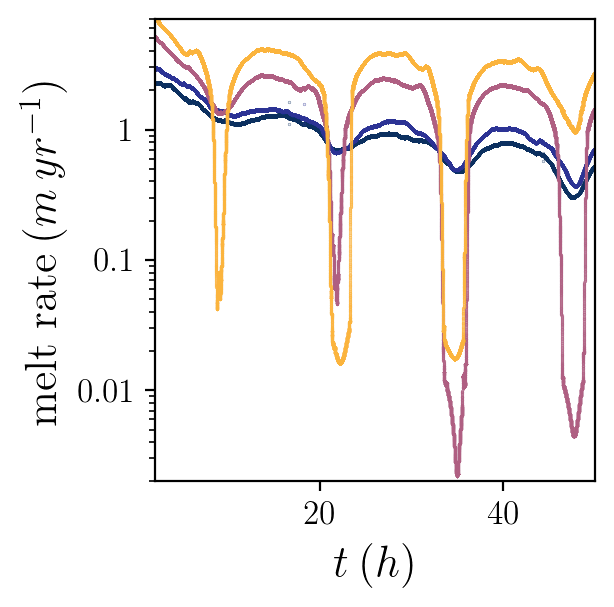
\includegraphics[trim={0 0cm 0 0},clip,width=\textwidth]{Figures/melt_cmp_dT_t.png}
    \end{minipage}%
    \begin{minipage}{0.4\textwidth}
        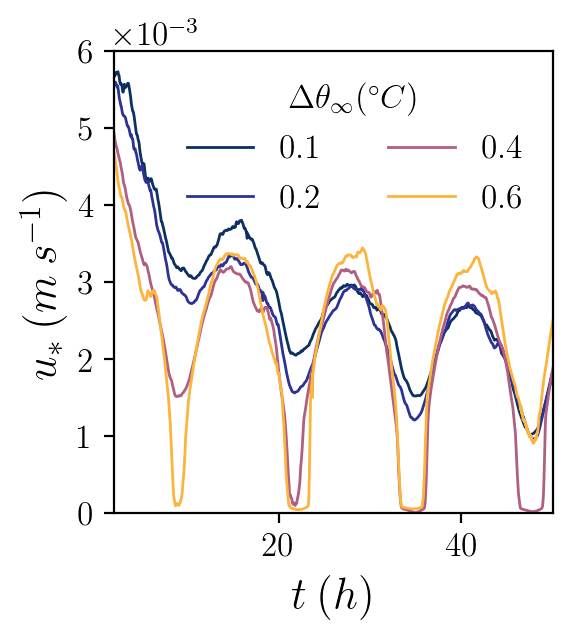
\includegraphics[trim={0 0cm 0 0},clip,width=\textwidth]{Figures/us_cmp_dT_t.png}
    \end{minipage}
    \begin{minipage}{0.4\textwidth}
        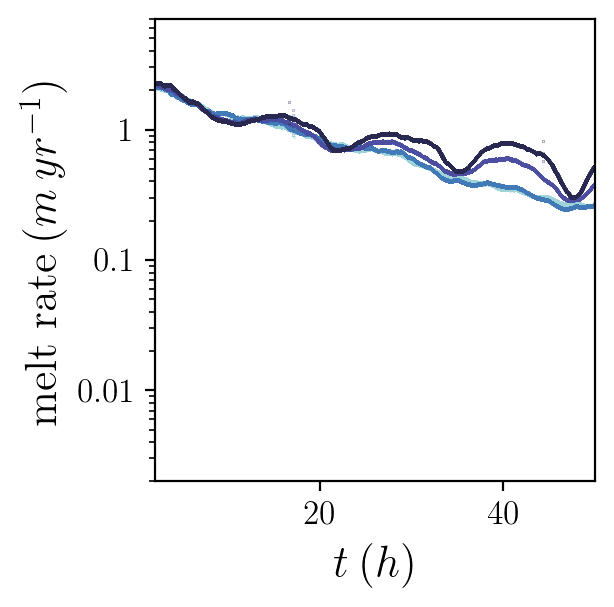
\includegraphics[trim={0 0cm 0 0},clip,width=\textwidth]{Figures/melt_cmp_dslope_t.png}
    \end{minipage}%
    \begin{minipage}{0.4\textwidth}
        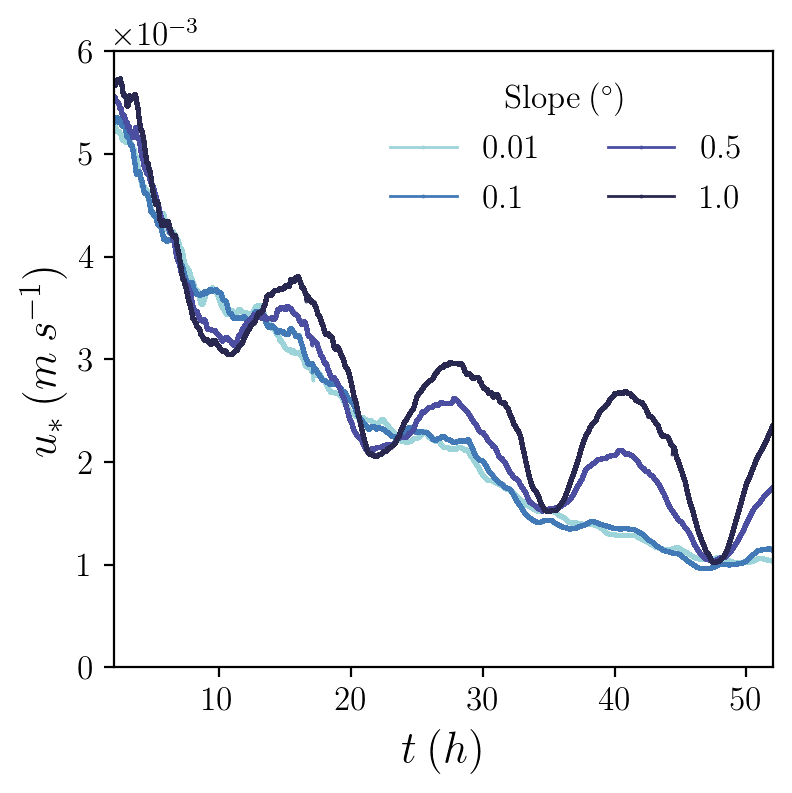
\includegraphics[trim={0 0cm 0 0},clip,width=\textwidth]{Figures/us_cmp_dslope_t.png}
    \end{minipage}
    \caption{Time evolution of (a,c) melt rate and (b,d) friction velocity for (a,b) thermal driving simulations and (c,d) varying slope simulations. Y-axis limits differ between panels, with the black curve representing the same simulation in all panels.}
    \label{fig:timeseries}
\end{figure}

We present depth-profiles of temperature, salinity, and velocity at the end of all simulations; Figure \ref{fig:dT_profiles} shows the results from the simulations in which we varied thermal driving, while Figure \ref{fig:dslope_profiles} shows those from the simulations with varying slope. All simulations show an evolution from the weakly stratified initial conditions to more strongly stratified conditions, particularly within the first 5 m of the ice-ocean interface (Figures \ref{fig:dT_profiles}b, \ref{fig:dslope_profiles}b). 

\begin{figure}[h!]
    \centering
    \begin{minipage}{0.33\textwidth}
        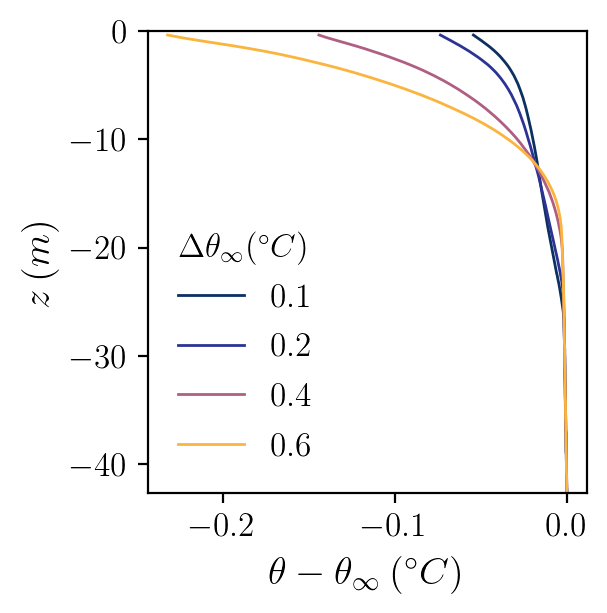
\includegraphics[trim={0 0cm 0 0},clip, width=\textwidth]{Figures/pt_cmp_dT_43h_tav13h_z_profile.png}
    \end{minipage}%
    \begin{minipage}{0.33\textwidth}
        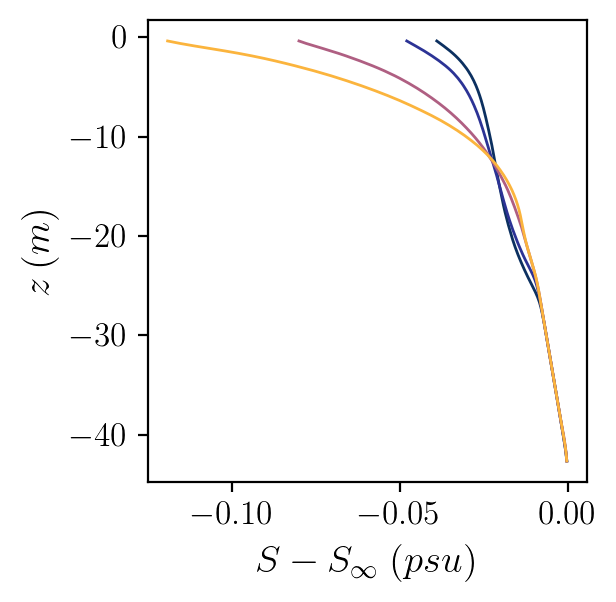
\includegraphics[trim={0 0cm 0 0},clip, width=\textwidth]{Figures/sa_cmp_dT_43h_tav13h_z_profile.png}
    \end{minipage}%
    \begin{minipage}{0.33\textwidth}
        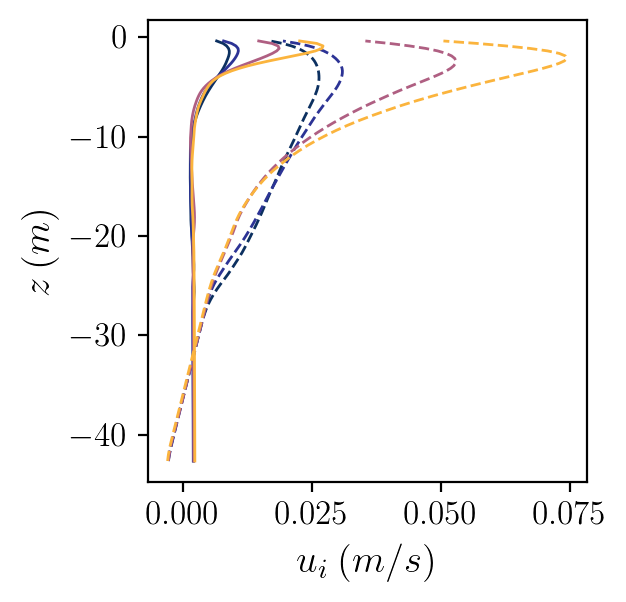
\includegraphics[trim={0 0cm 0 0},clip, width=\textwidth]{Figures/velocity_cmp_dT_43h_tav13h_z_profile.png}
    \end{minipage}
    \caption{Depth profiles of simulated properties as they vary with thermal driving, averaged over the last inertial period. (a) temperature relative to far-field temperature, (b) salinity relative to far-field salinity, and (c) velocity components. For panel (c), solid lines are in the positive y direction, dashed in positive x-direction (up-slope).}
    \label{fig:dT_profiles}
    % change colorbar label to \theta_\infty
\end{figure}

\begin{figure}[h!]
    \centering
    \begin{minipage}{0.33\textwidth}
        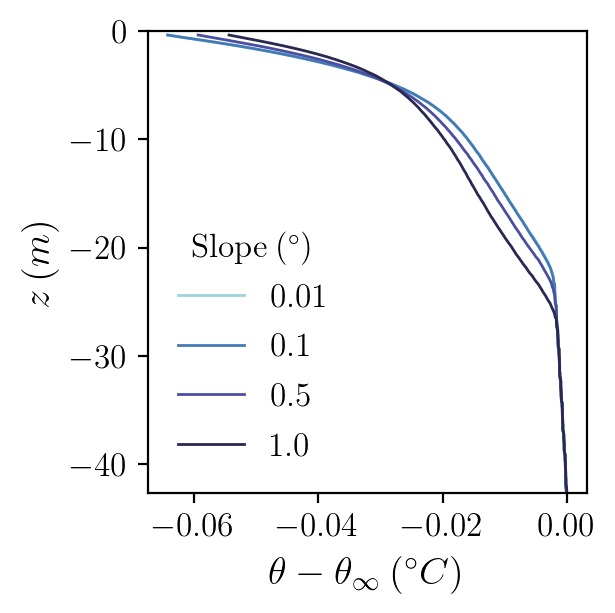
\includegraphics[trim={0 0cm 0 0},clip, width=\textwidth]{Figures/pt_cmp_dslope_43h_tav13h_z_profile.png}
    \end{minipage}%
    \begin{minipage}{0.33\textwidth}
        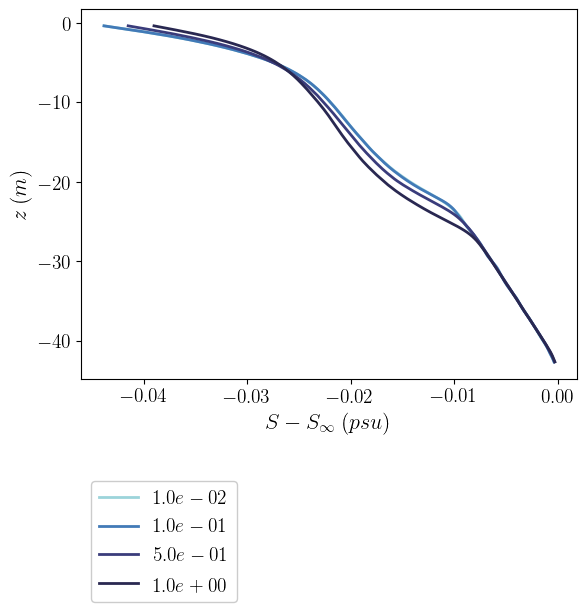
\includegraphics[trim={0 0cm 0 0},clip, width=\textwidth]{Figures/sa_cmp_dslope_43h_tav13h_z_profile.png}
    \end{minipage}%
    \begin{minipage}{0.33\textwidth}
        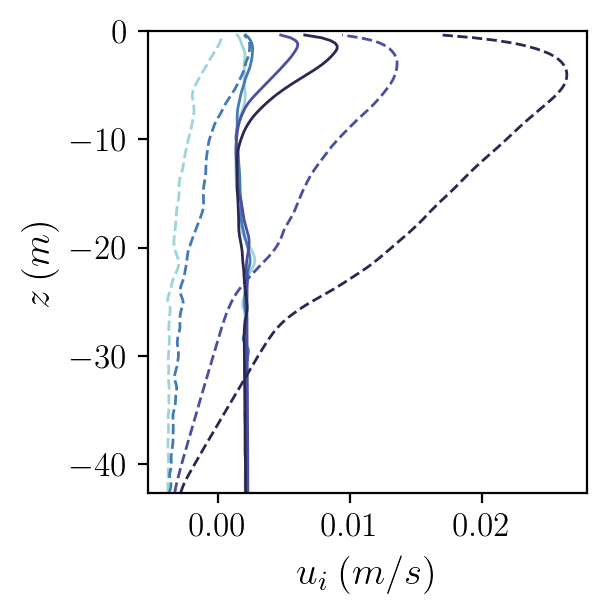
\includegraphics[trim={0 0cm 0 0},clip, width=\textwidth]{Figures/velocity_cmp_dslope_43h_tav13h_z_profile.png}
    \end{minipage}
    \caption{Depth profiles of simulated properties as they vary with slope, averaged over the last inertial period. (a) temperature relative to far-field temperature (b) salinity relative to far-field salinity (c) velocity components. For panel (c), solid lines are in the positive y direction, dashed in positive x-direction (up-slope). The black curve is common to both sets of simulations (see Figure \ref{fig:dT_profiles}).}
    \label{fig:dslope_profiles}
\end{figure}


% Description of velocity profiles
Ekman rotation near the boundary can be seen in all simulations (Figs. \ref{fig:dT_profiles}c and \ref{fig:dslope_profiles}c), but for more strongly sloped runs, buoyancy plays an increasingly strong role in driving the mean flow near the boundary. This effect can be seen most clearly by comparing the up-slope component of the flow within several meters of the ice-ocean interface across the slope-varying simulations (Figure \ref{fig:dslope_profiles}c). These mean buoyancy effects increase flow velocities on the order of a few cm s\textsuperscript{-1} as slope varies from 0.01$^{\circ}$ to 1.0$^{\circ}$ (Figure \ref{fig:dslope_profiles}c). Flow velocities near the boundary increase on the order of 10 cm s\textsuperscript{-1} as far-field thermal driving increases from 0.1 to 0.45$^{\circ}$C at 1$^{\circ}$ slope (Figure \ref{fig:dT_profiles}c). This velocity increase is attributed to changes in the magnitude of buoyancy forcing at the boundary, related to differences in melt rates. 

% BL depth
Stratification within the boundary layer increases with thermal driving (Figure \ref{fig:dT_profiles}a,b). Thus, the increase in melt-induced buoyancy fluxes with thermal driving dominates over the increase in shear induced by the buoyant flow. Conversely, stratification decreases with increasing slope, indicating that the increase in shear induced by the buoyant flow dominates over increase in melt-induced buoyancy fluxes with slope. The simulated boundary layer depth has a strong relationship with local thermal driving (i.e., the difference between IOBL temperature and the freezing point), reflecting entrainment of warm water below and setting mixing lengthscales  within the IOBL. Boundary layer depth is identified with the local maximum in the ratio of vertical to horizontal velocity variance (e.g., Figure S2). This definition of the IOBL can also be considered the depth to which shear originating at the boundary influences the flow. In none of the simulations is the boundary layer well-mixed with respect to either temperature or salinity. The boundary layer depth increases through time, reaching 15 -- 25 m at the end of the simulations. 

% TKE budget, shear
Shear production of turbulence dominates the TKE budget. The evolution of TKE ($E$) can be described by:
\begin{equation}
    \frac{dE}{dt} = F_{shear} + F_{buoy} + F_{trans} - \textrm{diss}
\end{equation}
Figure \ref{fig:tke_budget} shows several key terms in this budget for the variable slope simulations; the analogous figure for the thermal driving simulations is Figure S3 and shows similar patterns. Shear production ranges from $\sim 10^{-9} \textrm{--} 10^{-8}$ m\textsuperscript{2} s\textsuperscript{-3} with a maximum at the ice-ocean interface and local maxima in the upslope flow within 5 m of the boundary (Figure \ref{fig:tke_budget}a). The increase in TKE throughout the boundary layer as slope increases reflects this shear-induced turbulence (Figure \ref{fig:tke_budget}a).

% TKE budget, buoyancy
Buoyancy production of turbulence is 1 -- 2 orders of magnitude smaller than shear production, $\sim 10^{-10} \textrm{--} 10^{-9}$ m\textsuperscript{2} s\textsuperscript{-3}. In the sloped ice shelf, the buoyancy term can be broken into two components, the horizontal buoyancy fluxes that increase turbulence when oriented upslope and the vertical fluxes that decrease turbulence when ice is melting. Since our simulations only produce melting, the vertical component is always negative (dashed lines, Figure \ref{fig:tke_budget}b). Over the coarse of an inertial oscillation, the horizontal component of buoyancy production is generally positive when the mean flow is oriented upslope and negative when the the flow is oriented downslope. Interestingly, the time-averaged effect of a slope is destruction of turbulence near the boundary and production of turbulence near the base of the boundary layer (dotted lines, Figure \ref{fig:tke_budget}b). The net effect of both of the horizontal and vertical buoyancy components is the destruction of turbulence throughout the IOBL (solid lines, Figure \ref{fig:tke_budget}b), with the exception of the base of the IOBL where the horizontal buoyancy component augments entrainment. While these complexities are intriguing from a dynamical perspective, we do not explore them further here since the buoyancy term is not of leading-order in the TKE budget.

% TKE budget, transport
The transport term contains two components, advection of TKE due to pressure fluctuations and advection of TKE due to turbulence. The former is negligible, reaching maximum values on the order of $10^{-12}$ m\textsuperscript{2} s\textsuperscript{-3} while the latter increases turbulence at the boundary with oscillations of decreasing amplitude with distance from the boundary (Figure \ref{fig:tke_budget}c). 

% TKE budget, dissipation, tendency
Dissipation, the remaining term in the TKE budget, can be inferred from the remainder of these terms and the rate of change of TKE. In these simulations TKE is not in steady-state, with vertically-averaged $dE/dt$ ranging from $\sim 10^{XX} \textrm{--} 10^{XX}$ m\textsuperscript{2} s\textsuperscript{-3} in the IOBL. Thus, dissipation is on the same order as shear production but for many runs exceeds shear production as evidenced by declining TKE. 

\begin{figure}
    \centering
    \begin{minipage}{0.5\textwidth}
        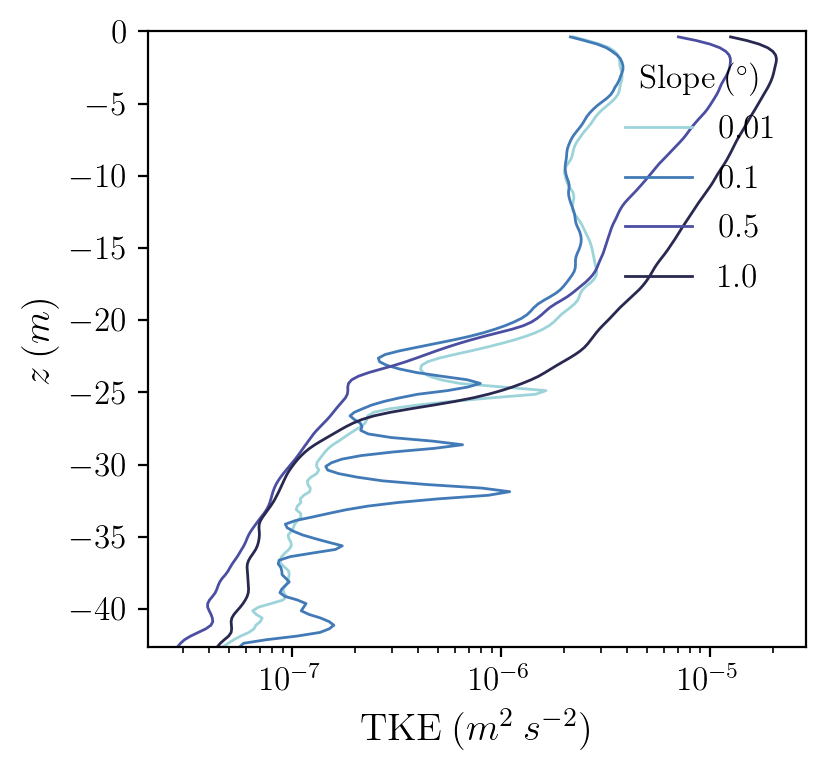
\includegraphics[trim={0 4.5cm 0 0},clip, width=\textwidth]{Figures/eres_cmp_dslope_43h_tav13h_z_profile.png}
    \end{minipage}%
    \begin{minipage}{0.5\textwidth}
        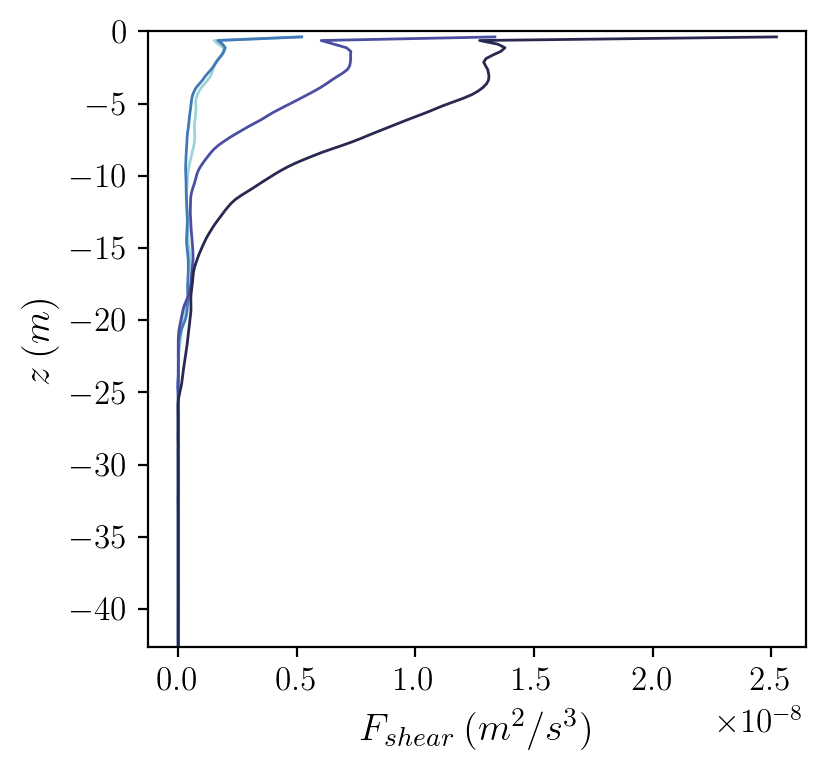
\includegraphics[trim={0 4cm 0 0},clip,width=\textwidth]{Figures/Fshear_cmp_dslope_43h_tav13h_z_profile.png}    
    \end{minipage}
    \newline
    \begin{minipage}{0.5\textwidth}
        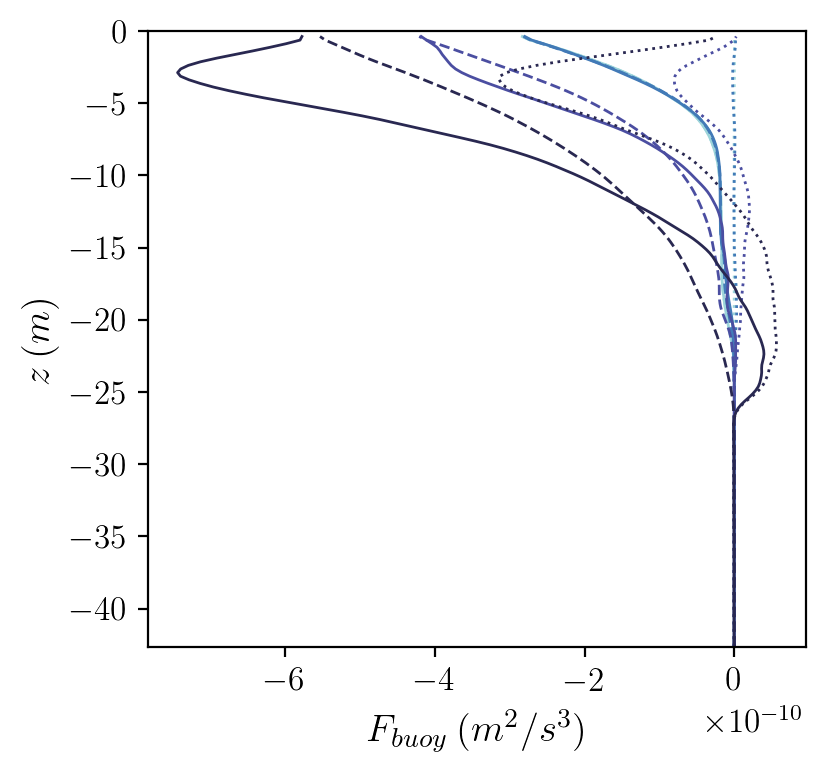
\includegraphics[trim={0 11cm 0 0},clip,width=\textwidth]{Figures/Fbuoy_cmp_dslope_43h_tav13h_z_profile.png}
    \end{minipage}%
    \begin{minipage}{0.5\textwidth}
        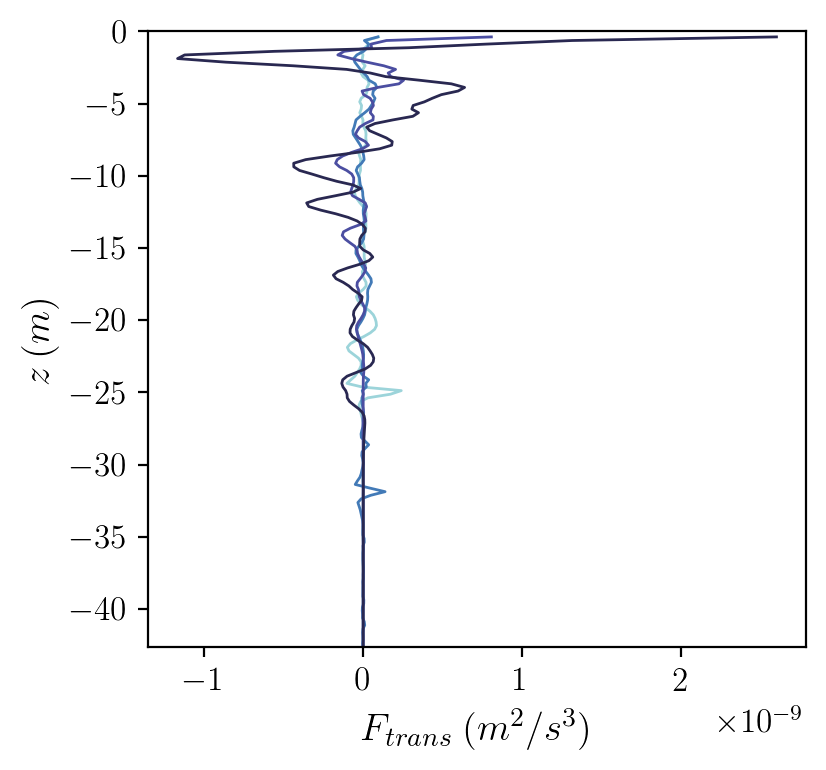
\includegraphics[trim={0 4cm 0 0},clip,width=\textwidth]{Figures/Ftrans_cmp_dslope_43h_tav13h_z_profile.png}
    \end{minipage}
    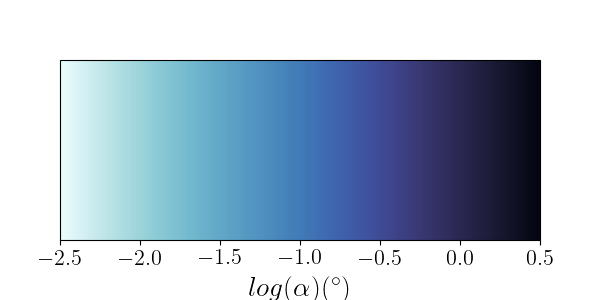
\includegraphics[width=0.4\textwidth,trim={1cm 0cm 1cm 5cm}, clip]{Figures/colorbar_slope.png}
    \caption{(a) Simulated turbulent kinetic energy for variable slope simulations averaged over the last inertial period and (b-d) turbulent kinetic energy production terms over the same period. (b) Shear production. (c) Buoyancy production. The total buoyancy production is shown with solid lines, vertical component dashed, and upslope component dotted. (d) TKE transport. Positive denotes production, negative destruction. Note that the x-axis scales differ between panels.}
    \label{fig:tke_budget}
    % Change x-axis label for buoyancy production terms
\end{figure}

% discuss turbulent structures
To demonstrate the simulated turbulent structures in this regime, we present horizontal and vertical cross-sectional  snapshots through the domain for the two slope end-members in Figure \ref{fig:cross-section}. Turbulent structures within the IOBL are consistent with propagating Holmboe shear instabilities under stable stratification \cite{carpenter_identifying_2010}. Shear is stronger within the IOBL than at the base of the IOBL due to the concentration of buoyant plume flow near the top of the IOBL. Consequently, the amplitude of these structures increases near the boundary for the more strongly-sloped simulations (Figures \ref{fig:cross-section}b,d). The difference in IOBL turbulence with slope is perhaps best seen in the turbulent structures at 1 m from the ice-ocean interface (Figure \ref{fig:cross-section}e,f). The structures become increasingly filamentous (i.e., near-wall streaks, e.g., \citeA{del_alamo_spectra_2003, hoyas_scaling_2006}) and coherent as slope and thus the buoyancy-driven current increase. Since the stratification decreases with increasing slope, the ratio of vertical to horizontal velocity variance also increases;  velocity fluctuations are less confined to the slope-parallel direction (Figure S2). 
% consider discussing entrainment here

\begin{figure}[h!]
    \centering
    \begin{minipage}{0.4\textwidth}
        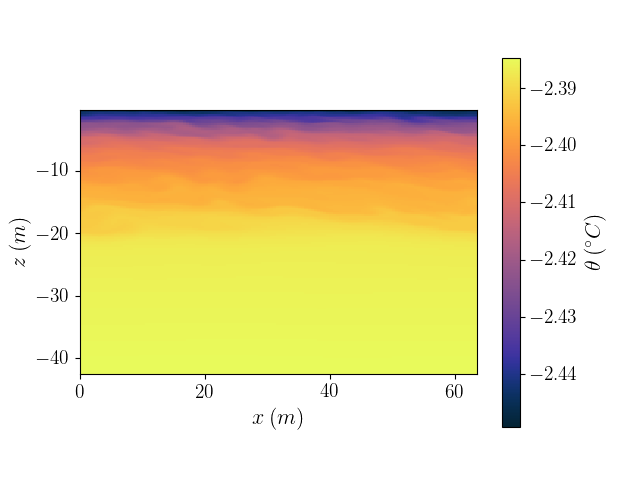
\includegraphics[trim={0 1cm 4cm 1cm},clip,width=\textwidth]{Figures/dslope2/pt_xz_y64_zmax42_t40.png}
    \end{minipage}%
    \begin{minipage}{0.55\textwidth}
        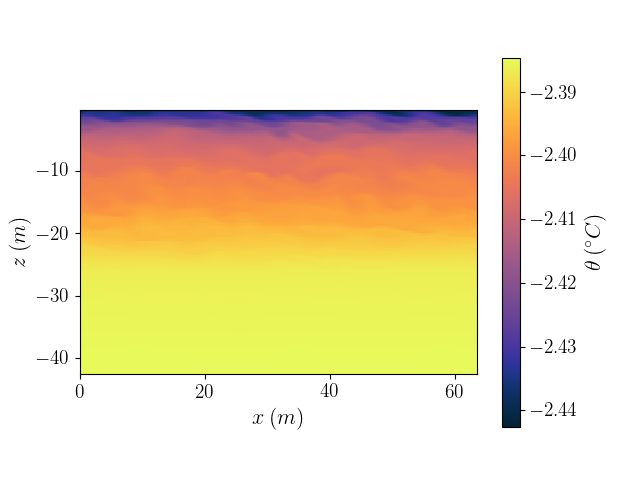
\includegraphics[trim={0 1cm 0 1cm},clip,width=\textwidth]{Figures/dT1/pt_xz_y64_zmax42_t40.png}
    \end{minipage}
    \begin{minipage}{0.4\textwidth}
        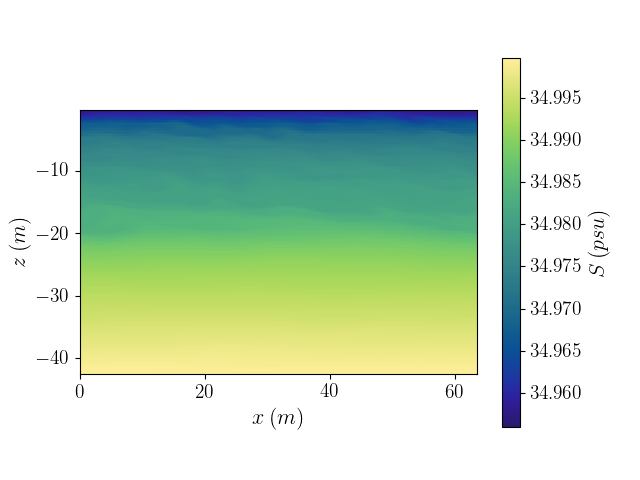
\includegraphics[trim={0 1cm 4cm 1cm},clip,width=\textwidth]{Figures/dslope2/sa_xz_y64_zmax42_t40.png}
    \end{minipage}%
    \begin{minipage}{0.55\textwidth}
        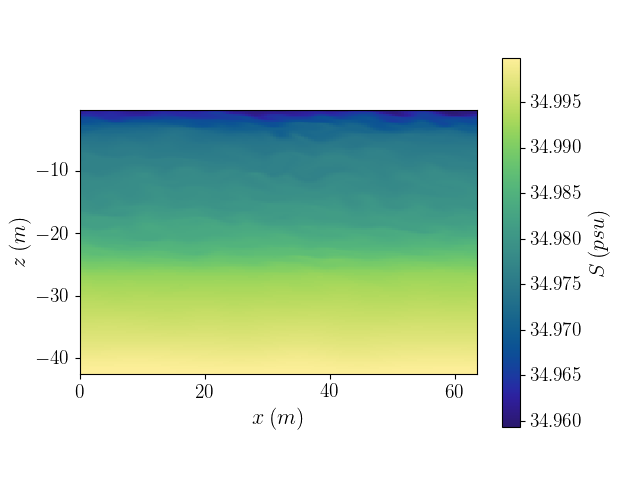
\includegraphics[trim={0 1cm 0 1cm},clip,width=\textwidth]{Figures/dT1/sa_xz_y64_zmax42_t40.png}
    \end{minipage}
    \begin{minipage}{0.45\textwidth}
        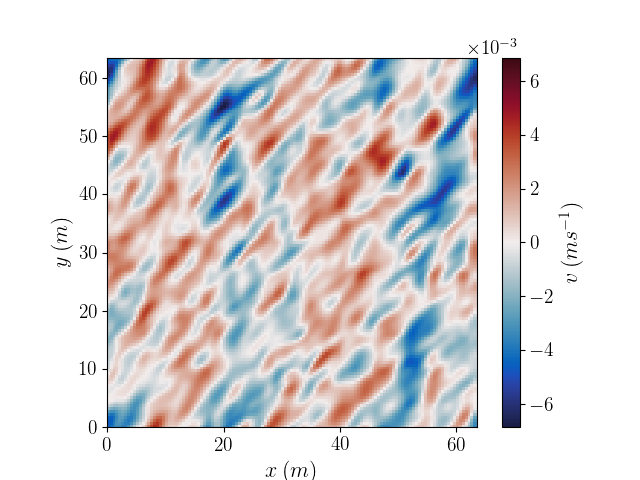
\includegraphics[trim={0 0cm 1cm 0},clip,width=\textwidth]{Figures/dslope2/v_xy_z1_zmax1_t40.png}
    \end{minipage}%
    \begin{minipage}{0.45\textwidth}
        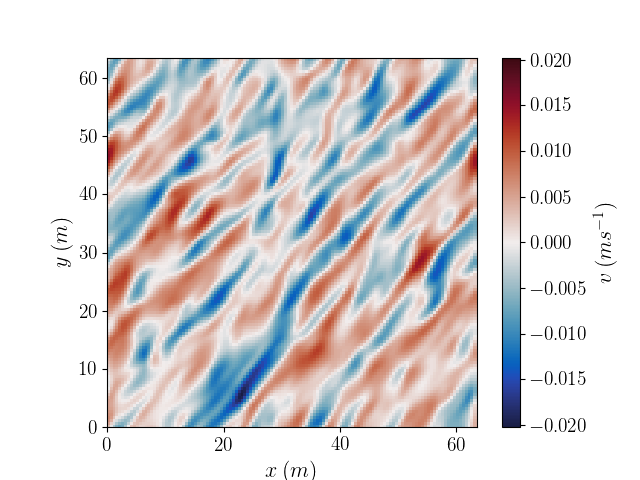
\includegraphics[trim={1cm 0cm 0cm 0},clip,width=\textwidth]{Figures/dT1/v_xy_z1_zmax1_t40.png}
    \end{minipage}%
    \begin{minipage}{0.05\textwidth}
    \hfill
    \end{minipage}
    \caption{Instantaneous flow structures observed at 40h in (a,c,e) 0.01$^{\circ}$ slope case and (b,d,f) 1$^{\circ}$ slope case. (a,b) Temperature in cross section mid-way through the y-axis. (c,d) Salinity in cross-section mid-way through the y-axis. (e,f) Cross-slope velocity fluctuations at 1 m below the ice-ocean interface. Note that the colorbar scale is smaller in (e) than (f).}
    % Add contours to a-d to show structures more clearly
    \label{fig:cross-section}
\end{figure}

% Melt rate relationship with inertial period
The dominant temporal frequency in melt rate is the inertial frequency, and the melt response to those oscillations is highly nonlinear. Maximum melt rates occur when the mean flow is oriented between the up-slope direction and the Coriolis-favored direction, and minimum melt rates roughly 180$^{\circ}$ opposed to that. These melt rate fluctuations correspond to fluctuations in TKE which are reflected in the friction velocity shown in Figure \ref{fig:timeseries}b. The dominant contribution to turbulence is shear production of TKE, which changes its distribution with depth as the mean flow profile evolves (Figure S3). During high-melt periods, the far-field flow is oriented up-slope and shear production of TKE is concentrated near the boundary (Figure \ref{fig:dT_profiles}c,d). During low-melt periods, the far-field flow is oriented down-slope and shear production of TKE is concentrated a few meters away from the boundary (Figure \ref{fig:tke_budget}b). 

% intermittent turbulence
Melt rate fluctuations increase in amplitude as thermal driving increases and as slope increases, which we attribute to the increasing importance of buoyancy forcing in driving a near-boundary plume and thus determining the depth-distribution of shear. At higher slopes ($\geq 0.5^{\circ}$), inertial oscillations enhance shear mixing first near the boundary; this mixing front then propagates to the base of the mixed layer over a few hours (not shown). The two simulations associated with the highest thermal driving values, and the highest near-boundary stratification, experience a hiatus in turbulence during the down-slope flow period. This can be seen in the dramatic reduction in friction velocity (i.e., shear stress) at the ice interface (Figure \ref{fig:timeseries}b). Thus, in our simulations rotational effects cause intermittency in turbulence when the IOBL is sufficiently stratified. We discuss this intermittency further in Section \ref{disc:dyn}.

\begin{figure}[h!]
    \centering
    \begin{minipage}{0.4\textwidth}
        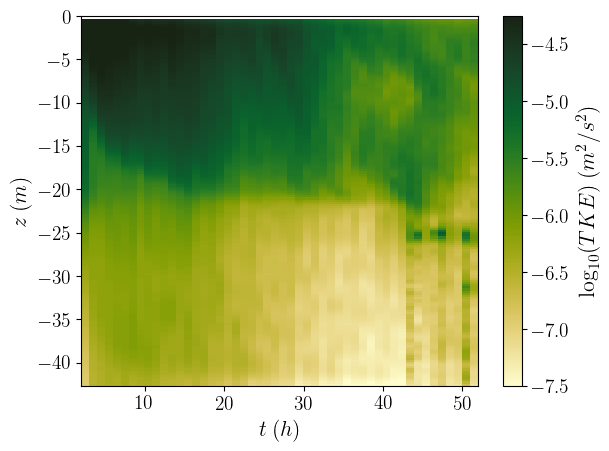
\includegraphics[trim={0 0cm 3cm 0cm},clip,width=\textwidth]{Figures/dslope2/e_hovmoller.png}
    \end{minipage}%
    \begin{minipage}{0.5\textwidth}
        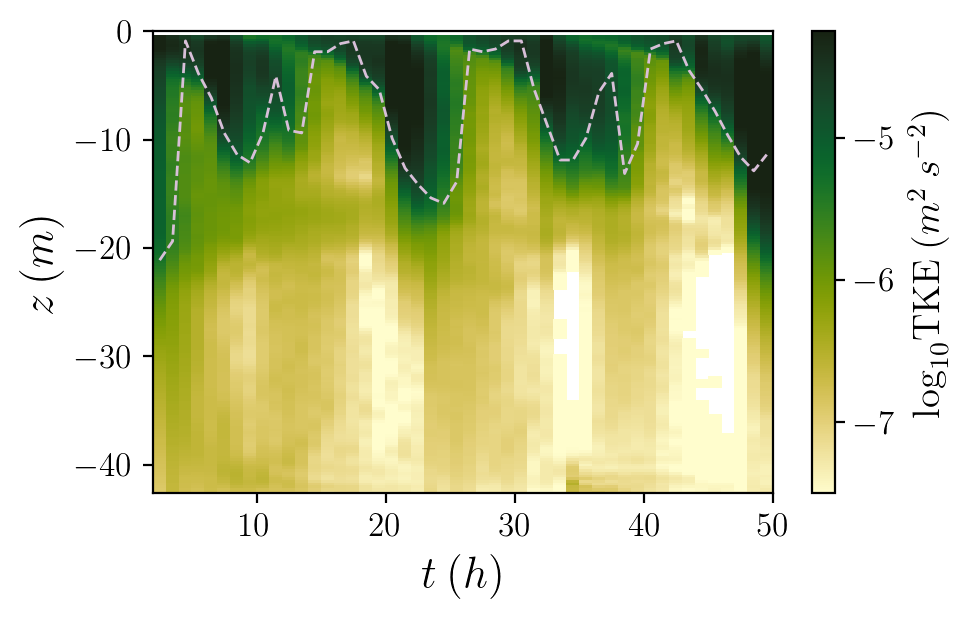
\includegraphics[trim={0 0cm 0 0cm},clip,width=\textwidth]{Figures/dT4/e_hovmoller.png}
    \end{minipage}
    \begin{minipage}{0.4\textwidth}
        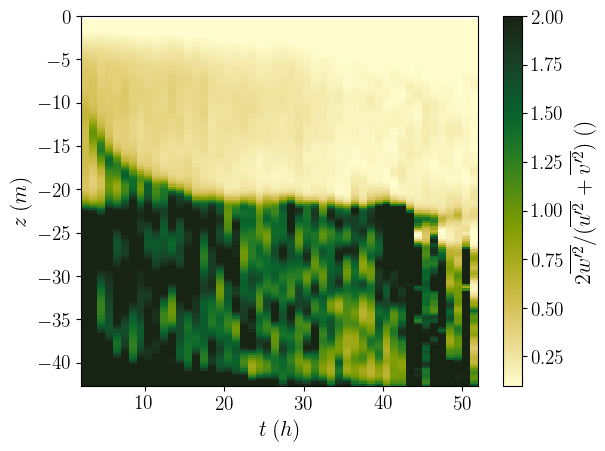
\includegraphics[trim={0 0cm 3cm 0cm},clip,width=\textwidth]{Figures/dslope2/vel_var_ratio_hovmoller.png}
    \end{minipage}%
    \begin{minipage}{0.5\textwidth}
        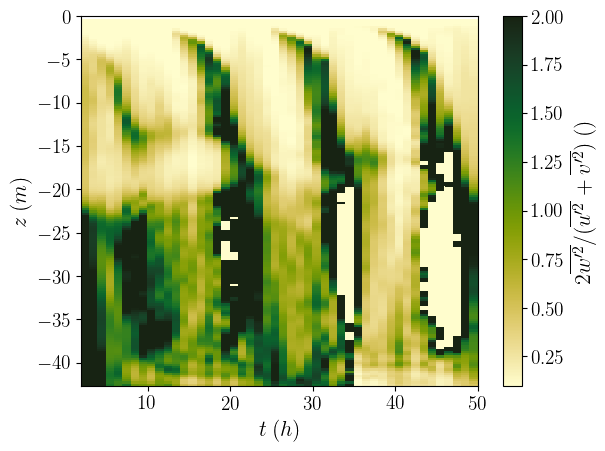
\includegraphics[trim={0 0cm 0 0cm},clip,width=\textwidth]{Figures/dT4/vel_var_ratio_hovmoller.png}
    \end{minipage}
    \caption{Example of turbulent intermittency as seen in (a,b) TKE and (c,d) vertical velocity variance. (a,c) A non-intermittent case: 0.1$^{\circ}C$ thermal driving, 0.01$^{\circ}$ slope. (b,d) An intermittent case: 0.45$^{\circ}C$ thermal driving, 1$^{\circ}$ slope.}
    \label{fig:intermittency}
\end{figure}


% Melt rate sensitivity to thermal driving
Time-averaged melt rates are roughly linear with thermal driving (Figure \ref{fig:melt_sensitivity}a). The derived, time-averaged thermal exchange coefficient (described in Section \ref{meth:tcm}) is fairly insensitive to thermal driving. The thermal exchange coefficient during the last 12 hours of the simulations is between 0.005 and 0.006 for the simulated range of thermal driving values. During the first 12 hours of the simulation, simulated thermal exchange coefficients are 0.008 due to weaker stratification near the interface, higher friction velocities, and greater TKE. The derived thermal exchange coefficient decreases somewhat in the high thermal driving cases due to pronounced periods of low melt as TKE declines with increasing stratification. 

\begin{figure}[h!]
    \centering
    \begin{minipage}{0.5\textwidth}
        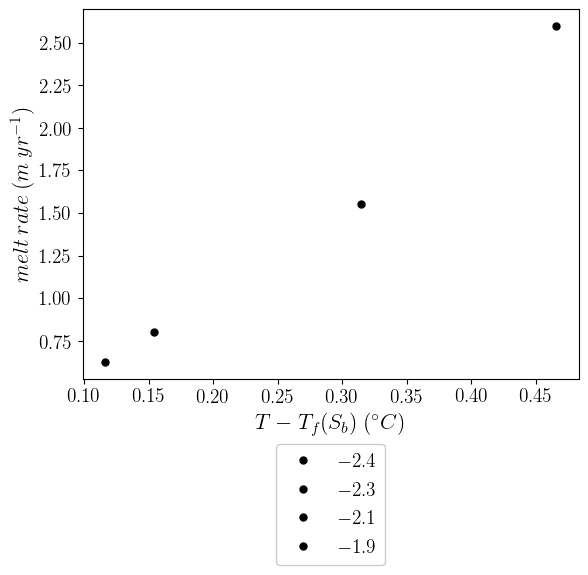
\includegraphics[trim={0 3.5cm 0 0},clip,width=\textwidth]{Figures/melt_dT_tav12.png}
    \end{minipage}%
    \begin{minipage}{0.5\textwidth}
        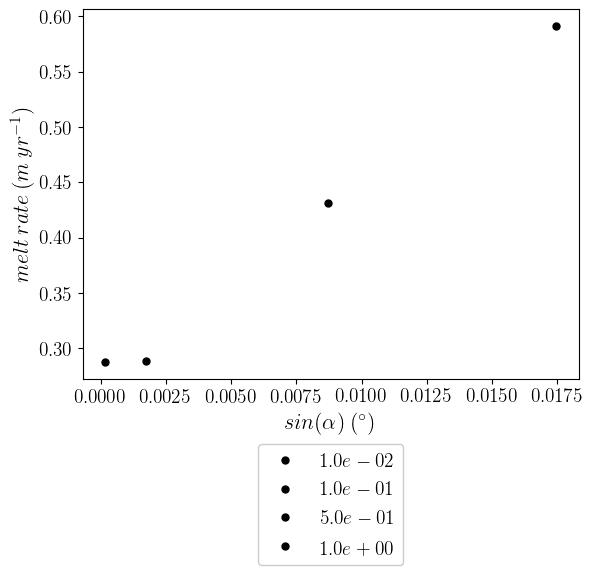
\includegraphics[trim={0 3.5cm 0 0},clip,width=\textwidth]{Figures/melt_dslope_tav12.png}
    \end{minipage}
    \begin{minipage}{0.5\textwidth}
        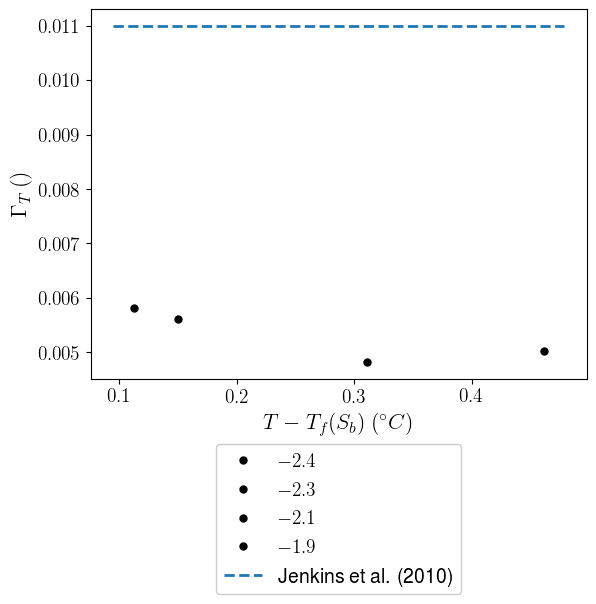
\includegraphics[trim={0 4.1cm 0 0cm},clip,width=\textwidth]{Figures/gammaT_dT_tav12_zlim2.png}
        \vspace{0.7cm}
    \end{minipage}%
    \begin{minipage}{0.5\textwidth}
        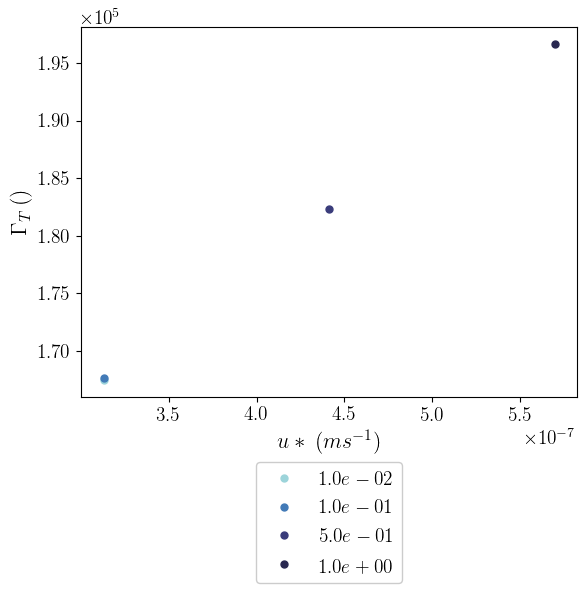
\includegraphics[trim={0 3.4cm 0 0cm},clip,width=\textwidth]{Figures/gamma_T__us__dslope_tav12_tlim52.png}
        \centering
        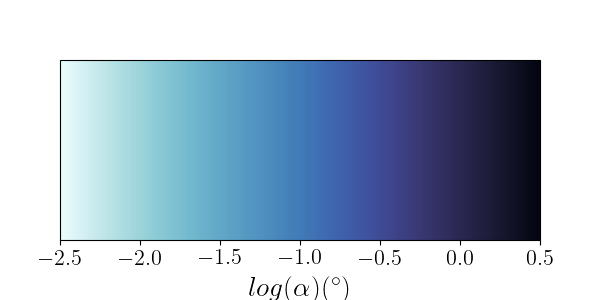
\includegraphics[width=0.7\textwidth,trim={1cm 0cm 1cm 5cm}, clip]{Figures/colorbar_slope.png}
    \end{minipage}
    \caption{(a) Melt rate vs. thermal driving. (b) Melt rate vs. slope. (c) Thermal exchange coefficient vs. far-field thermal driving for thermal driving simulations. Dashed line denotes the value recommended by \citeA{jenkins_observation_2010}. (d) Thermal exchange coefficient vs. friction velocity for sloped simulations. Note the difference in y-axis limits from (c). The 0.01$^{\circ}$ and 0.1$^{\circ}$ slope cases are overlapping.}
    \label{fig:melt_sensitivity}
\end{figure}

% Melt sensitivity to slope
There is also a linear relationship between melt rate and ice-shelf basal slope, with threshold-like behavior at slopes less than 0.01$^{\circ}$. This threshold behavior in melting in the two lowest-slope cases is attributable to similar friction velocities (Figure \ref{fig:melt_sensitivity}d) arising from similar IOBL velocities and turbulence  (Figure \ref{fig:dslope_profiles}c,d). This behavior is discussed in more detail in Section \ref{disc:prm}. The differences in derived thermal exchange coefficient are not pronounced as slope varies, on the order of a 10\% change as slope increases from 0.01$^{\circ}$ to 1$^{\circ}$ (Figure \ref{fig:melt_sensitivity}d). Variability in the thermal exchange coefficient with slope is largely determined by differences in friction velocity between simulations (Fig. \ref{fig:melt_sensitivity}d) while there is a smaller ($\sim$20\%) opposite effect from decreasing interfacial thermal driving with increasing slope (not shown). These differences in friction velocity arise from higher IOBL velocities and turbulence at higher slopes (Figure \ref{fig:dslope_profiles}c,d). 

% Scaling for flux profiles
The relatively narrow range of conditions simulated here suggests that a depth-dependent shape function for scalar fluxes could be formulated. The distance from the interface is scaled by the Ekman depth:
\begin{equation}
    d_E = (2 K_e)^{1/2} |f_3|^{-1/2}
\end{equation}
where $K_{b}$ is the mean bulk viscosity in the turbulent boundary layer assuming the total fluxes follow Fick's law:
\begin{equation}
    \overline{w'\mathbf{u}'} = K_{b} d\mathbf{u}/dz
\end{equation}
$K_e$ profiles are shown in Figure S4. 

% Scaling heat flux profiles with thermal driving
The linear scaling of melt rate with thermal driving suggests a linear scaling of heat flux profiles with thermal driving. We find that this scaling largely collapses the four thermal driving profiles, with some deviation from this shape for the run that experiences intermittent turbulence (Figure \ref{fig:heatflux_profiles}c). The shape of these profiles can be reasonably approximated by a linear decrease in the scaled heat flux with scaled depth over the boundary layer (Figure \ref{fig:heatflux_profiles}c). Scalar fluxes decline near the boundary for the 1$^{\circ}$ slope cases, a feature that we discuss further in Section \ref{disc:prm}. Since the IOBL is fully turbulent (with the exception of some intermittency discussed below), the sub-grid diffusivities of momentum, heat and salt closely resemble one another (Figure S5). The vertical salt flux profiles are shown in Figure S6 and have a very similar shape to the vertical heat flux profiles.


\begin{figure}[h!]
    \centering
    \begin{minipage}{0.5\textwidth}
        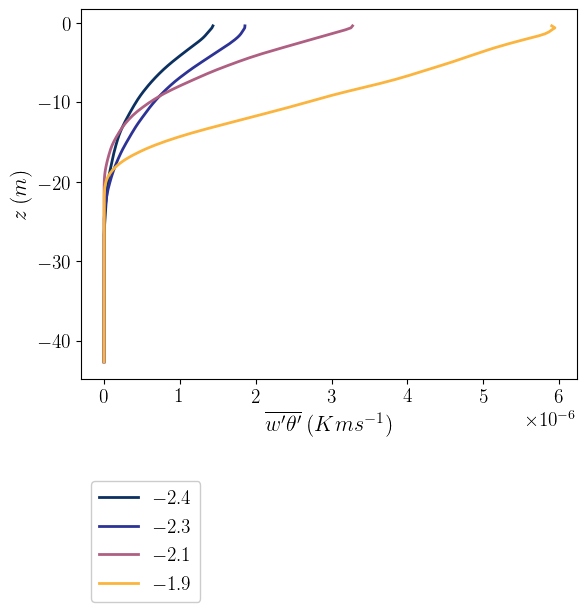
\includegraphics[trim={0 4cm 0 0},clip,width=\textwidth]{Figures/heatflux_cmp_dT_44h_tav12_z_profile.png}
    \end{minipage}%
    \begin{minipage}{0.5\textwidth}
        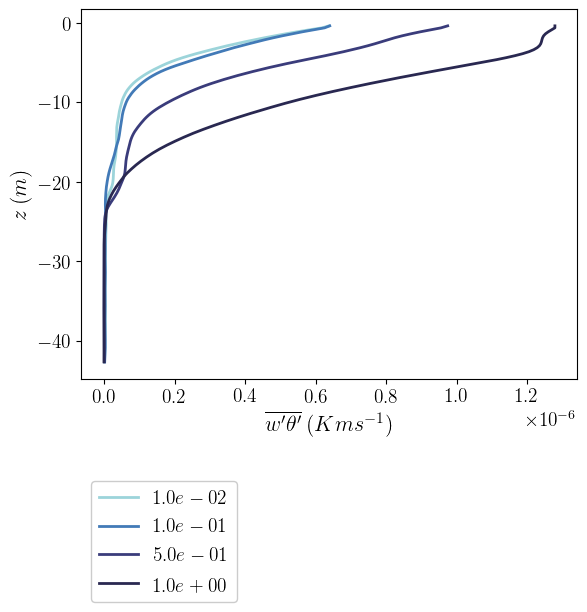
\includegraphics[trim={0 4cm 0 0},clip,width=\textwidth]{Figures/heatflux_cmp_slope_46h_tav12_z_profile.png}
    \end{minipage}
    \begin{minipage}{0.5\textwidth}
        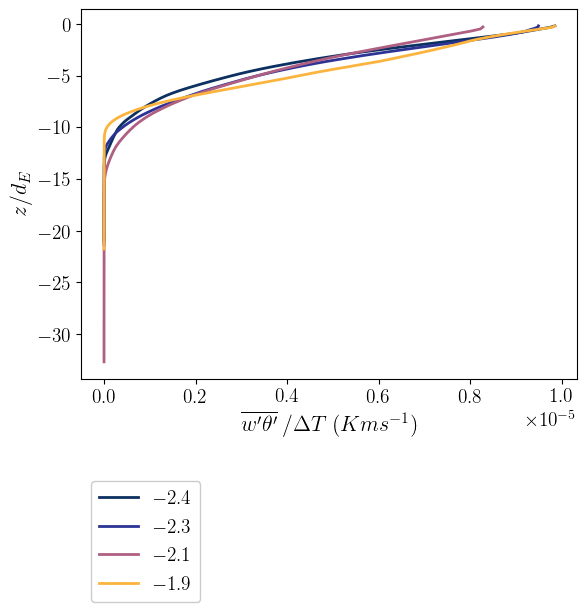
\includegraphics[trim={0 4cm 0 0},clip,width=\textwidth]{Figures/heatflux_cmp_dT_43h_tav13_dTscale_z_profile.png}
        \centering 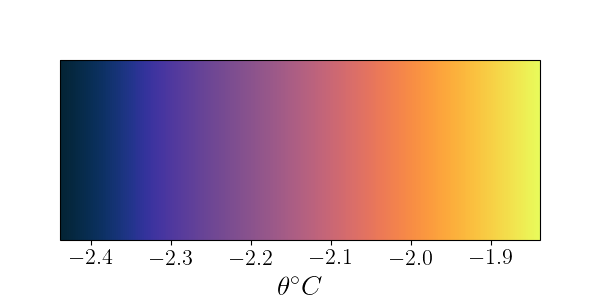
\includegraphics[width=0.7\textwidth,trim={1cm 0cm 1cm 5cm}, clip]{Figures/colorbar_thermal_driving.png}
    \end{minipage}%
    \begin{minipage}{0.5\textwidth}
        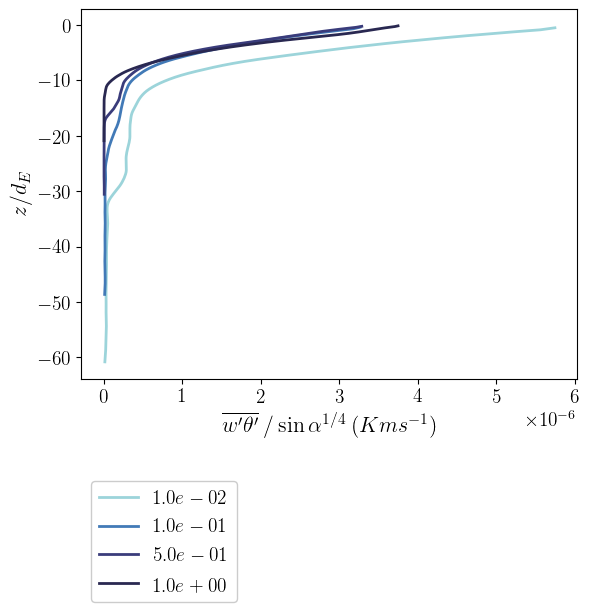
\includegraphics[trim={0 4cm 0 0},clip,width=\textwidth]{Figures/heatflux_cmp_slope_46h_tav13_slopescale_z_profile.png}
        \centering 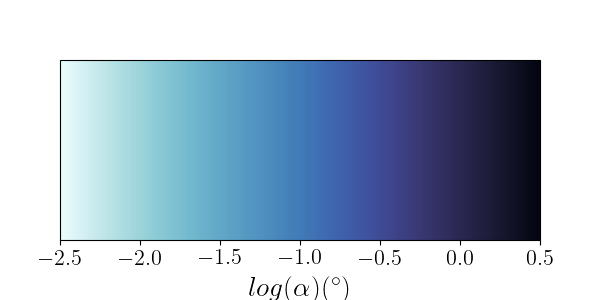
\includegraphics[width=0.7\textwidth,trim={1cm 0cm 1cm 5cm}, clip]{Figures/colorbar_slope.png}
    \end{minipage}
    \caption{Vertical profile of heat flux averaged over the last inertial period for (a,c) temperature cases and (b,d) slope cases. (a,b) are in physical units while (c,d) are scaled by the Ekman depth, far-field thermal driving, and slope. The black curve is represents the same simulation in all panels.} 
    %Consider replacing (d) with scaling by sin\alpha
    %Change scaled vertical axis limits to 0-40
    %Change all to centered on 43h and averaged 13h
    \label{fig:heatflux_profiles}
\end{figure}

% Scaling heat flux profiles with slope
Despite melt rates scaling reasonably well with the basal slope ($\sin \alpha$), the vertical heat flux profile does not, showing a much lower sensitivity to slope ($\sin^{1/4}\alpha$, Figure \ref{fig:heatflux_profiles}d). We also find that the Ekman depth is a poor predictor of boundary layer depth. This may be due to the depth-variable shear induced by buoyancy which is not reflected in the depth-mean IOBL bulk viscosity used to compute the Ekman depth. 
%It is interesting that the boundary layer depths of the thermal driving cases at 1$^{\circ}$ slope scale similarly with the Ekman depth despite the differences in buoyancy of the IOBL (Figure \ref{fig:heatflux_profiles}c). It suggests that the bulk viscosity in the IOBL, used to compute the Ekman depth, is a poor predictor of entrainment as slope varies. 

% momentum flux profiles
By looking at the variation of momentum flux with depth shown in Figure \ref{fig:momflux_profiles}, we can examine the relative contributions of interfacial drag and buoyant acceleration of the IOBL to the velocity profiles shown in Figure \ref{fig:dT_profiles}c,e and \ref{fig:dslope_profiles}c. Since the mean velocity is oriented both upslope (+$u$) and cross-slope (+$v$), positive $\overline{u'w'}$ and $\overline{v'w'}$ close to the interface indicate slowing of the current due to drag whereas negative $\overline{u'w'}$ and $\overline{v'w'}$ a few m below the interface through much of the boundary layer indicate buoyant acceleration of the IOBL. The amplitude of momentum fluxes increases with slope and thermal driving consistent with increases in IOBL velocity and TKE. Intermittency in turbulence also changes the shape of momentum flux profile, displacing momentum peaks closer to the surface as the IOBL shoals (pink curve, Figure \ref{fig:momflux_profiles}a). 

\begin{figure}[h!]
    \begin{minipage}{0.5\textwidth}
        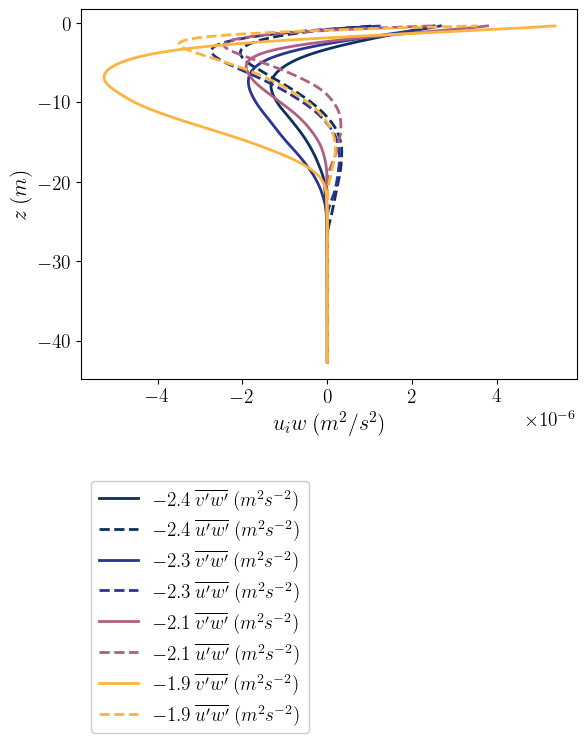
\includegraphics[trim={0 7.5cm 0 0},clip,width=\textwidth]{Figures/momflux_cmp_dT_44h_tav12_z_profile.png}
        \centering 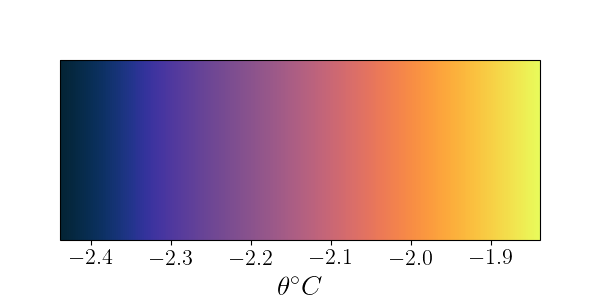
\includegraphics[width=0.7\textwidth,trim={1cm 0cm 1cm 5cm}, clip]{Figures/colorbar_thermal_driving.png}
    \end{minipage}%
    \begin{minipage}{0.5\textwidth}
        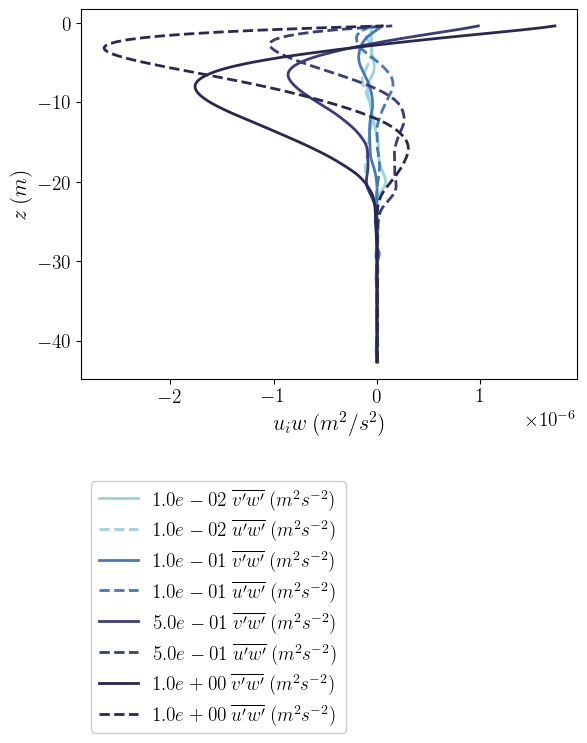
\includegraphics[trim={0 7.5cm 0 0},clip,width=\textwidth]{Figures/momflux_cmp_dslope_46h_tav12_z_profile.png}
        \centering 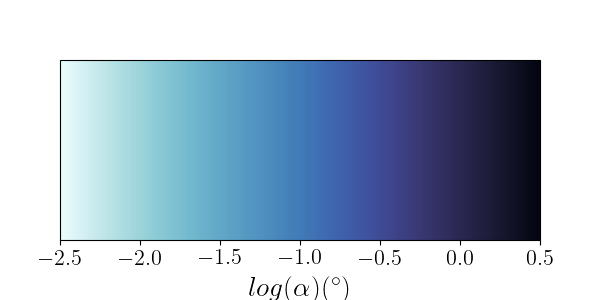
\includegraphics[width=0.7\textwidth,trim={1cm 0cm 1cm 5cm}, clip]{Figures/colorbar_slope.png}
    \end{minipage}
    \caption{Momentum flux averaged over the last inertial period for (a) thermal driving cases and (b) slope cases. Momentum flux is expressed in two components:  $\overline{u'w'}$ (dashed) and $\overline{v'w'}$ (solid). Positive flux denotes upward flux (i.e., drag) and }
    \label{fig:momflux_profiles}
    % change x-axis labels to \overline{u_i'w'}
\end{figure}

\section{Discussion}\label{disc}

\subsection{IOBL turbulence} \label{disc:dyn}

In the simulations presented here, turbulence declines throughout the course of the simulation; for a few highly stratified cases becoming intermittent. The relationship between stable stratification, shear, and the persistence of turbulence remains an open question \cite{zonta_stably_2018}. Thus, it is not possible a priori to determine whether the level of turbulence simulated by this LES model is appropriate for the regime space we have sampled. While we did conduct model validation against a stably stratified atmospheric boundary layer test case (see Section \ref{meth:tcm}), the degree of stratification at the boundary in that case did not approach that simulated in the sub-ice configuration. Fundamentally, we cannot guarantee that our LES is not overly dissipative such that the TKE generated by the resolved dynamics is lost too quickly relative to real-world sub-ice settings. 

Excess dissipation could arise either through the sub-grid scheme or the model numerics. We found a rapid loss of turbulence in PALM simulations when a dynamic Smagorinky turbulence closure was used, which is consistent with previous studies on the limited applicability of the standard Smagorinsky turbulence closure to strongly stratified flows due to the strong anisotropy of these flows \cite{flores_analysis_2011, jimenez_large-eddy_2005}. This motivated our adoption of the AMD turbulence closure scheme. However, we found that the buoyancy term suggested by \citeA{abkar_large-eddy_2017} had an unrealistically high magnitude in the vicinity of the ice base where gradients are large. We neglected this term as \citeA{vreugdenhil_stratification_2019} found it to be negligible, but our unrealistic solution for this term suggests that AMD scheme may not perform optimally at the resolution employed here, which is significantly lower than that used by \citeA{vreugdenhil_stratification_2019}. 

Strongly stratified turbulence has been associated with intermittent turbulence \cite{nieuwstadt_direct_2005, wiel_cessation_2012}, though there are also numerical experiments that fail to produce intermittency even under strongly stable stratification \cite{arya_buoyancy_1975, komori_turbulence_1983}. This is not the first study to find the emergence of intermittent turbulence in stably stratified, sub-ice settings \cite{vreugdenhil_stratification_2019}. Flow relaminarization occurs periodically in our most strongly stratified simulations; stratification coincident with high thermal driving and high melt rates. \citeA{donda_collapse_2015} have argued that, in strongly stratified flows, the cessation of turbulence is transient provided there are sufficiently large perturbations. This is consistent with our finding that the temporal variability in shear over inertial oscillations provides a sufficient perturbation to reinitiate turbulence. Our simulations approach a gradient Richardson number of 0.25, which is considered to be the approximate value at which turbulence neither grows nor decays \cite{rohr_growth_1988, holt_numerical_1992}. Thus, fluctuations in TKE are plausible at the simulated levels of stratification and shear. However, when turbulence is intermittent, as it is in this study, the application of LES may be inappropriate due to its inherent horizontal averaging over laminar and turbulent regions \cite{stoll_large-eddy_2008}. Thus, our results at the highest thermal-driving values should be interpreted with caution. 

In this study, we did not attempt to reproduce observed conditions at a particular ice-shelf location due to the difficulties of matching unobserved far-field forcings and the exclusion of tides from our simulations for ease of interpretation. Nonetheless, it appears as though well-mixed boundary layers are simulated for a narrower range of conditions in simulations than in observations. The background flow chosen in these simulations is quite strong at 20 cm s\textsuperscript{-1} and thermal driving is relatively low such that we expected to produce a well-mixed boundary layer as is observed in melting regions of the Filchner-Ronne Ice Shelf \cite{nicholls_oceanographic_2001}. However, observations to date are insufficient to provide reliable predictions of IOBL stratification \cite{malyarenko_synthesis_2020}. The observational picture is quite nuanced with a range of stratification observed even within one ice shelf (e.g., \citeA{hattermann_two_2012}). 

Our simulations are certainly missing some sources of TKE present in ice-shelf cavities which could modify IOBL structure and mixing efficiency. These simulations did not include tides, which provide perturbations to the mean velocity that enhance melt rates and entrainment, especially at Filchner-Ronne \cite{makinson_modeling_1999, makinson_influence_2011, mueller_tidal_2018}. While internal gravity waves arise in LES, they may be of smaller amplitude and play a lesser role in mixing than they would in a real ice-shelf settings due to the absence of large-scale external forcings such as tides and storms, seafloor topography, as well as possible resonance with the cavity geometry \cite{gwyther_cold_2020}. Enhanced drag at the ice-shelf base could increase shear production of TKE; however under strong stratification, surface roughness elements may suppress turbulence rather than enhance it \cite{ohya_wind-tunnel_2001}. 

% Consider discussing boundary layer depth and entrainment

% Consider leading this section with the discussion of shear-driven turbulence
Shear-driven turbulence within the IOBL plays a central role in determining vertical heat fluxes and thus melt rates. In these simulations the destruction of TKE by the stabilizing buoyancy flux is two orders of magnitude smaller than shear production of TKE throughout the IOBL. Our finding that shear production of TKE dominates over the buoyancy term is consistent with \citeA{davis_turbulence_2019} who found that shear production was an order of magnitude greater than buoyancy destruction of TKE in the IOBL below Larsen C Ice Shelf. 

The flux Richardson number, $\text{Ri}_f$, the ratio of buoyancy flux to shear-driven TKE production, provides a measure of mixing efficiency. The simulated $\text{Ri}_f$ values of 0.05 -- 0.1 are well below the critical $\text{Ri}_f$ of $\sim\!0.2$, indicating that we are in the regime in which mixing efficiency ($\text{Ri}_f$) decreases with increasing stratification ($\text{Ri}_g$) \cite{armenio_investigation_2002, peltier_mixing_2003}. This is consistent with our finding that the thermal exchange coefficient decreases for the high thermal driving cases which also achieve stronger IOBL stratification.


\subsection{Evaluating melt sensitivity and turbulent flux representations in ocean models}\label{disc:prm}

\subsubsection{Insights into melt sensitivity to ocean conditions}

% Argument for validity of findings in non-steady conditions
The decline in IOBL turbulence discussed in Section \ref{disc:dyn} results in declining melt rates, making it difficult to evaluate the relationship between melting and far-field conditions at steady state, which would provide the most direct path to assessing melt rate sensitivity to ocean conditions. As discussed in \citeA{jenkins_simple_2016}, achieving steady-state solutions in simulations may require prescribing large-scale gradients in temperature. We have not included these large-scale gradients in our simulations, but this may be an avenue for future work. However, we believe that our transient solutions do provide some indications of how melt rates and boundary layer properties depend on ocean temperature and ice-shelf slopes. One justification for this belief is that the simulated sensitivity of melt rate to ocean temperature and slope remains consistent through time during the last two inertial periods simulated. Furthermore, we find similar sensitivities of melt rate to IOBL temperature and velocity in simulations with different initial conditions at times for which IOBL conditions are statistically similar.

% sensitivity of melt rate to temperature
The linear relationship we find between far-field ocean temperature and melt rates is consistent with some previous studies \cite{rignot_rapid_2002}. It's worth noting that our simulations do not capture the large scale increase in overturning circulation that accompanies an increase in far-field thermal driving. The quadratic relationship between melt rate and thermal driving in \citeA{holland_response_2008} is a function of both a linear relationship between the local, far-field thermal driving and melt rate and a linear relationship between far-field thermal driving and friction velocity. The former relationship is addressed by this study and agrees with \citeA{holland_response_2008}; the latter is only partially captured by the increase in IOBL velocity due to an increase in buoyancy while the far-field velocity is unchanged. In contrast, in sea ice settings this sensitivity was found to be significantly smaller with an exponent of 0.38 \cite{ramudu_large_2018}. 

To some extent, this linear relationship between far-field thermal driving and melt rate is embedded in the parameterization of heat fluxes employed at the ice base in these simulations. Specifically, the melt rate is prescribed to have a linear dependence on the thermal driving using the temperature in the first model layer, see Equation \ref{eq:melt_flux}. However, the level of stratification near the ice base, the buoyant acceleration of the IOBL plume and the transport of heat from depth to the IOBL can mediate this relationship between \textit{far-field} temperature and melt rates, and yet the dependence from these simulations is still fairly linear.  

% sensitivity of melt rate to slope
The finding that slopes as low as 0.5$^{\circ}$ significantly influence melt rates is not unexpected from a consideration of momentum balance, but may be an underappreciated aspect of IOBL simulation in Antarctic ice-shelf settings. The linear relationship between ice-shelf slope and melt rate suggests a stronger dependence at very low slopes than that found by \cite{mondal_ablation_2019} using Direct Numerical Simulations at higher slopes ($m \propto \sin^{2/3}\alpha$). Further investigation would be needed beyond the small number of simulations presented here to diagnose this discrepancy. 

% sensitivity of melt rate to slope, at very low slopes
The threshold-like behavior in melt rates at very low slopes is not predicted by geostrophic balance between Coriolis and buoyancy forcing, which dictates a linear relationship between $\sin\alpha$ and IOBL velocity. This threshold behavior could be produced if any additional buoyant acceleration produced by the small increase in slope from 0.01$^{\circ}$ to 0.1$^{\circ}$ increases dissipation, resulting in a negative feedback on IOBL turbulence. From a dynamical perspective, this may be an interesting target for more highly resolved LES in the near-boundary region. However, this threshold is located at low enough slopes that it is likely not of significance to melt rate parameterization for coarse-resolution ocean models, so we do not devote further attention to it here. 


\subsubsection{Thermal exchange coefficient}

% Methodology for evaluating thermal exchange coefficient
The thermal exchange coefficient as computed using Equation \ref{eq:gamma} at 0.25m below the ice-ocean interface (the uppermost grid cell) differs from that which would be implemented by coarse-resolution models or derived from oceanographic observations, both of which only know ocean properties on the order of 1 m below the ice-ocean interface. Thus, we compute a thermal exchange coefficient using ocean properties 2 m below the ice-ocean interface. We substitute the friction velocity computed by Equation \ref{eq:tau} with one computed using a quadratic drag law from the velocity at 2 m and the applied drag coefficient, consistent with modeled drag implementations. This approach allows the closest comparison between the thermal exchange coefficient indicated by these simulations and that currently parameterized in ocean models. 

% discussion of low thermal exchange coeff in all runs
The thermal exchange coefficients used in these simulations are less than the value of 0.011 derived from observations \cite{jenkins_observation_2010}. There are two main factors that contribute to this result. The first is the choice of the parameterization of fluxes at the ice-ocean interface (i.e., over sub-meter scales). We chose a stability-dependent parameterization in which the buoyancy forcing from melting enters through the Monin-Obukhov lengthscale. We believe there is a stronger case for the flux parameterization we implement than for a constant thermal exchange coefficient in light of the success of Monin-Obukhov Similarity Theory \cite{monin_basic_1954}, the work of McPhee \cite{mcphee_air-ice-ocean_2008} and the depth-scaling of scalar fluxes in a more highly resolved sub-ice LES \cite{vreugdenhil_stratification_2019}. However, we acknowledge that more validation of these parameterizations is needed. The second contributing factor is declining simulated TKE, which results in a $\sim$50\% reduction of thermal exchange coefficients over the coarse of these simulations. 

% thermal exchange coeff, thermal driving
Our results also suggest a modest decline in the thermal exchange coefficient at higher thermal driving, which may lead to a sub-linear relationship between thermal driving and melt rate at higher thermal driving values. Due to the limitations of our LES modeling discussed in Section \ref{disc:dyn}, we cannot recommend under what range of thermal driving values a reduced thermal exchange coefficient may be appropriate. Given the climatic importance of accurately simulating high thermal driving regimes associated with dynamic ice-shelf thinning, this may be a fruitful avenue for future work.

% thermal exchange coeff, slope
The relationship between the thermal exchange coefficient and slope can be reduced to a linear relationship between thermal exchange coefficient and friction velocity. Our simulations are too few to evaluate whether a similar relationship holds when the source of friction velocity changes is the background flow rather than the slope. LES of sea ice melting does support this linear relationship between thermal exchange coefficient and friction velocity XX \cite{ramudu_large_2018}. In any case, the changes in the thermal exchange coefficient with slope were small, only 10\% between 0$^{\circ}$ and XX$^{\circ}$ cases. This suggests that, if a coarse-resolution simulation predicts friction velocity accurately, a melt parameterization with a constant thermal exchange coefficient may be adequate in Antarctic ice-shelf settings. Thus, the burden of melt projection accuracy may fall more heavily on parameterizing or resolving buoyant flow than on improving the slope-dependence in the parameterization of scalar fluxes (i.e., improving Equation \ref{eq:melt_flux}).


\subsubsection{Depth-dependence of turbulent fluxes}

% Need for modified vertical mixing parameterization
There is reason to believe that improving ice-shelf basal melt projections using ocean models will require not only an accurate melt parameterization but also an improved vertical mixing scheme. \citeA{jenkins_shear_2021} demonstrated significantly different IOBL characteristics when the K-profile Parameterization (KPP) was used in contrast to a low- or high-order turbulence closure scheme. The bulk viscosity simulated by our LES model shows better agreement with the viscosity solutions from \citeA{jenkins_shear_2021} employing the low- and high-order turbulence closure schemes than that employing KPP (his Figure 3). Thus, this study offers additional support for the use of a more sophisticated turbulence closure scheme or modified KPP scheme in sub-ice settings.

% model resolution challenges
A complication in melt parameterization of slope effects is the differential ability of ocean models and their vertical grid configurations to capture IOBL flow. We find that this buoyant flow is concentrated in the uppermost 10 m, with peak velocities as close as 3 m from the interface. This flow is unlikely to be resolved by most ocean models, which have typical vertical resolutions near the interface of 10s m though some model configurations are reaching $\sim$1 m resolutions \cite{gwyther_cold_2020}. This then raises important questions about the parameterization of ice-ocean interface scalar and momentum fluxes. If the buoyancy-driven boundary current is unresolved in most coarse-resolution ocean models, then the friction velocity as computed from a quadratic drag law and the velocity at the first grid cell is likely to underestimate the true friction velocity. For instance, in our simulations a friction velocity computed from the far-field velocity is $\sim$XX\% greater than the interfacial friction velocity. Thus, more accurate melt rate projections may result prescribe a depth-dependent parameterization of vertical scalar and momentum fluxes to provide some sensitivity of melt rates to model resolution. 

% scalar flux profiles
Our depth-dependent shape function for scalar fluxes agrees with the turbulent scalar flux parameterization of \citeA{mcphee_dynamics_1987}, which features a linear increase from 0 at the boundary layer depth to the flux at the surface. The simulations with slopes of 1$^{\circ}$ diverge from this linear behavior within a few m from the boundary. We attribute this to boundary effects that reduce TKE and bulk diffusivity close to the boundary, reminiscent of the constant flux layer predicted by Monin-Obukhov Similarity Theory \cite{monin_basic_1954}. This shape function for scalar fluxes through the IOBL should be explored under a broader range of conditions to determine whether this linear scaling is broadly applicable and whether vertical mixing parameterizations need to account for a constant flux layer. It's worth noting that any implementation of these depth-dependent scalar fluxes necessitates an inequality between the vertical heat and salt fluxes from the top model grid cell and the heat and salt fluxes associated with melting. Thus, the closure of those budgets will likely involve horizontal scalar fluxes as well.

% scalar flux profiles vs. slope - does not exist
Assuming one's vertical mixing parameterization accurately predicts the bulk viscosity of the IOBL, the Ekman depth scaling is a moderately strong predictor for IOBL depth as the thermal driving changes but a weak predictor for IOBL depth as slope changes. Given the presence of intermittency in our 1$^{\circ}$ slope simulations and relatively small differences in IOBL depth among our simulations, further work is needed to understand entrainment processes for the IOBL so that a depth-dependent shape function for scalar and momentum fluxes can be established. 

A depth-dependent function for momentum is also necessary in ice-shelf settings given that strong stratification causes momentum fluxes to significantly deviate from the quadratic drag function typically employed in ocean models. Even in the absence of ice-shelf slope, the near-interface stratification significantly decreases drag \cite{garcia-villalba_turbulence_2011, mcphee_revisiting_2008}. The addition of an ice-shelf slope to ocean models that do not fully resolve a buoyant plume further complicates the parameterization of momentum fluxes at the ice-ocean interface. A depth-dependent shape function for momentum fluxes which may prescribe negative (downward) momentum fluxes at the top grid cell below ice shelves for typical ocean model resolutions (see Figure \ref{fig:momflux_profiles} at, e.g., 5 m depth). In other words, the momentum boundary condition may need to accelerate the flow at the boundary (at least in the up-slope direction) to produce more accurate shear-driven mixing in the resolved portion of the domain when the buoyant plume is unresolved. 

\section{Conclusion}


\section{Acknowledgements}

This work was funded by the U.S. Department of Energy (DOE), Office of Science, Biological and Environmental Research, and Advanced Scientific Computing Research programs. Carolyn Begeman received funding for this work from a Chick Keller Postdoctoral Fellowship through the Center for Earth and Space Sciences at Los Alamos National Laboratory. Computing resources were provided by the Los Alamos National Laboratory Institutional Computing Program, which is supported by the U.S. Department of Energy National Nuclear Security Administration under Contract No. 89233218CNA000001.

\newpage
\bibliography{references}

\end{document}